\documentclass[12pt]{report} % Times New Roman, 12pt
%\usepackage{gscale_thesis_singlespace} % Single spaced thesis
\usepackage{gscale_thesis_doublespace} % Double spaced thesis
\usepackage{fancyheadings} % Header and footer styling
\usepackage[numbers]{natbib} % Bibliography formatting
\usepackage{setspace} % Allows double spacing but skips headers/footers
\setcounter{tocdepth}{1} % Limits the TOC to chapter and section names

% Additional packages
\usepackage{graphicx} % Allows the inclusion of figures
\usepackage{subcaption} % Allows captions to be added to subfigures
\usepackage[justification=centering]{caption} % Centres caption text
\usepackage{array} % Used for table formatting
\newcolumntype{P}[1]{>{\raggedright\let\newline\\\arraybackslash\hspace{0pt}}m{#1}}
\usepackage{booktabs} % Fancy-style tables
\usepackage{longtable} % Allows for tables that are more than one page long
\usepackage{float} % Better figure placement control
\usepackage{enumerate} % Numbered lists
\usepackage[shortlabels]{enumitem} % For controlling enumerate labels
\usepackage[shortcuts]{extdash} % Allows manual hyphenation of hypenated words
\usepackage{amsmath} % Non-standard math symbols
\usepackage{amsfonts} % Extended fonts for mathematics

\usepackage[hidelinks]{hyperref} % Linking to LaTeX labels and external URLs

\numberwithin{equation}{section} % Numbers equations based on their section

% Additional packages
\usepackage{xcolor}
\numberwithin{equation}{section}       % Numbers equations based on their 
									   %   section
\usepackage[normalem]{ulem}			   % Strikeout and advanced emphasis

% ********************************
\definecolor{codegreen}{rgb}{0,0.6,0}  % Custom code colours
\definecolor{codegray}{rgb}{0.5,0.5,0.5}
\definecolor{codepurple}{rgb}{0.58,0,0.82}
\definecolor{backcolour}{rgb}{0.95,0.95,0.92}


\usepackage{listings}				   % For code
\lstdefinestyle{mystyle}{
    backgroundcolor=\color{backcolour},   
    commentstyle=\color{magenta},
    keywordstyle=\color{codegreen},
    numberstyle=\tiny\color{codegray},
    stringstyle=\color{codepurple},
    basicstyle=\ttfamily\scriptsize,
    breakatwhitespace=false,         
    breaklines=true,                 
    captionpos=b,                    
    keepspaces=true,                 
    numbers=left,                    
    numbersep=5pt,                  
    showspaces=false,                
    showstringspaces=false,
    showtabs=false,                  
    tabsize=2
}
\lstset{style=mystyle}
% ********************************

\newif\ifcomments\commentstrue

\ifcomments
\newcommand{\authornotes}[3]{\textcolor{#1}{[#3 ---#2]}}
\newcommand{\todo}[1]{\textcolor{red}{[TODO: #1]}}
\else
\newcommand{\authornotes}[3]{}
\newcommand{\todo}[1]{}
\fi

\newcommand{\wss}[1]{\authornotes{blue}{SS}{#1}}
\newcommand{\jc}[1]{\authornotes{red}{JC}{#1}}
\newcommand{\ds}[1]{\authornotes{cyan}{DS}{#1}}

% *******Custom commands**********

%Cards
\newcommand{\card}[3]{
  \begin{center}
    \begin{tabular}{||p{0.8\linewidth}||}
	\hline
	\textbf{Name}: {\textbf{#1}} \\ \hline
	\textbf{Problem being solved}: #2 \\ \\
	Relevant artifacts: #3 \\
	\hline
    \end{tabular}
  \end{center}
}

\newcommand{\cardifact}[2]{
  \begin{center}
    \begin{tabular}{||p{0.8\linewidth}||}
	\hline
	\textbf{Name}: {\textbf{#1}} \\ \hline
	\textbf{Description}: #2 \\
	\hline
    \end{tabular}
  \end{center}
}

%Shortcuts
\def\smithea{Smith et al.}
\def\sfs{softifacts}
\def\sf{softifact}
\def\SFS{Softifacts}
\def\SF{Softifact}
\def\gp{GamePhysics}
\def\gb{GlassBR}
\def\sw{SWHS}
\def\np{NoPCM}
\def\sp{SSP}
\def\pr{Projectile}


%Figures
\newcommand{\fig}[3]{
  \begin{figure}
    #1
  \caption{#2}
  \label{#3}
  \end{figure}
}

%Tables
%\newcolumntype{P}[1]{>{\centering\arraybackslash}p{#1}}
% ********************************
\begin{document}
\title{Generating Jupyter Notebooks in Drasil}
\halftitle{Generating Jupyter Notebooks in Drasil} % 60 Characters Max. 
%Including Spaces

\author{Ting-Yu Wu}
\shortauthor{Ting-Yu Wu} % Used for page header

\dept{Department of Computing and Software}
\field{Computing and Software} % What field your thesis is in (e.g. Software 
%Engineering)

\prevdegreeone{B.Sc. (Information \& Computer Engineering),\\Chung Yuan 
Christian University, Taoyuan, Taiwan}
\prevdegreetwo{B.Sc.} % Just your degree's field

\submitdate{April 2023} % Use the month's full spelling e.g. November
\copyrightyear{2023} % Year you are submitting this, usually your graduation 
%year

\doctype{Report} % ``Report'' or ``Thesis'' or whatever you need
\degree{Masters of Engineering} % The degree you get when you submit this
\degreeabbrv{M.Eng.}
\principaladviser{Dr. Spencer Smith and Dr. Jacques Carette} % Your Supervisor
 % LaTeX variables for preface pages/headers
    
\beforepreface % Half title page, title page, declaration page   
  \prefacesection{Lay Abstract}

A lay abstract of not more 150 words must be included explaining the key goals and contributions of the thesis in lay terms that is accessible to the general public.  % Lay Abstract
  \prefacesection{Abstract}
Drasil is a framework that generates software, including code, documentation, software requirement specification, user manual, and axillary files. Recently, the Drasil team has been interested in expanding its knowledge to solve higher-order ODEs. In this research, for single higher-order linear ODEs, the Drasil framework can solve them without manually extracted information. For higher-order nonlinear ODEs, the Drasil framework can solve them with manually extracted information.

Firstly, we design a flexible and reusable structure to store ODE information based on conventional mathematical knowledge. This makes it possible to reuse ODE information for documentation and for code generation. Secondly, we provide a commonality analysis of four external ODE solver libraries. The analysis includes how they solve the ODE, what algorithms they use, and what options they provide for different types of output. Thirdly, we enable the Drasil Code Generator to solve nonlinear higher-order ODEs with some manually extracted information. We created a new case study, Double Pendulum, that has a system of higher-order ODE. Further, we solve the Double Pendulum example numerically via external libraries. Lastly, for single higher-order ODEs, the Drasil Code Generator can generate code without manually extracted information.

This research accomplishes three main goals. Firstly, we capture the knowledge of linear ODE in a flexible and reusable structure. Secondly, we expand the Drasil capability to solve higher-order ODEs with/without manually written equations. Solving single higher-order linear ODEs does not require manually extracted information. To solve nonlinear ODEs, manually extracting information from the original ODE is still required. The last one is removing the duplicated information caused by the implementation of solving ODEs. % Abstract
  %\thispagestyle{empty}
\null\vfill
\begin{center}
%\textbf{Dedications}
%\linebreak
\textsl{Your Dedication \\ Optional second line}
\end{center}
\vfill
 % Dedication
  \prefacesection{Acknowledgements}

I would like to express my deepest appreciation to my supervisors, Dr.\ Spencer Smith and Dr.\ Jacques Carette. With their guideline, I could break a complex puzzle into smaller pieces and accomplish them one by one. I spent 90\% of my time in remote learning, but the quality of knowledge I received beyond learning in-person. My supervisors quickly adapted the work rhythm during the pandemic, and I greatly benefited from it.

Special thanks to my friend and colleague Jason Balaci for answering my questions and providing excellent suggestions for learning.

I am also thankful to my parents for supporting me in pursuing my second master's degree. Although my parents received very little education, they supported me in pursuing higher education mentally and financially.

Lastly, I want to thank Sophie for motivating me out of the bottom rock of my life.  % Acknowledgements
  \referencepages % Table of Contents, List of Figures, List of Tables
  \prefacesection{Notation, Definitions, and Abbreviations}
\ds{TODO: Update this}
\section*{Notation}
\begin{description}[font=\rmfamily\bfseries, leftmargin=3cm, style=nextline]
	\item[$A \leq B$] A is less than or equal to B
\end{description}

\section*{Definitions}
\begin{description}[font=\rmfamily\bfseries, leftmargin=3cm, style=nextline]
	\item[\SF] A portmanteau of `software' and `artifact'. The term refers to 
	any of the artifacts (documentation, code, test cases, build instructions, 
	etc.) created during a software project's development.
\end{description}

\section*{Abbreviations}
\begin{description}[font=\rmfamily\bfseries, leftmargin=3cm, style=nextline]
	\item[QA] Quality Assurance
	\item[SI] Syst\`eme International d'Unit\'es
	\item[SRS] Software Requirements Specification
\end{description}
  \academicstatement{academicachievementdeclaration}
\afterpreface
  
  
  \chapter{Introduction}
\ds{Introduce the term softifact somewhere in here}

\ds{Pain points and problems come first, then solution is docs, then problems 
with writing docs, then the rest of this.}
Documentation is good\citep{??}, yet it is not often prioritized on software
projects. Code and other software artifacts say the same thing, but to different
audiences - if they didn't, they would be describing different systems.

Take, for example, a software requirements document. It is a human-readable
abstraction of *what* the software is supposed to do. Whereas a design document
is a human-readable version of *how* the software is supposed to fulfill its
requirements. The source code itself is a computer-readable list of instructions
combining *what* must be done and, in many languages, *how* that is to be
accomplished.

[Put in figures of an example from GlassBR/Projectile here, showing SRS, DD, and
code versions of the same knowledge]

[Figure] shows an example of the same information represented in several
different views (requirements, detailed design, and source code). We aim to
take advantage of the inherent redundancy across these views to distill a single
source of information, thus removing the need to manually duplicate information
across software artifacts.

Manually writing and maintaining a full range of software artifacts (i.e.
multiple documents for different audiences plus the source code) is
redundant and tedious. Factor in deadlines, changing requirements, and other
common issues faced during development and you have a perfect storm for
inter-artifact syncronization issues.

How can we avoid having our artifacts fall out of sync with each other?
Some would argue "just write code!" And that is exactly what a number of other
approaches have tried. Documentation generators like Doxygen, Javadoc, Pandoc,
and more take a code-centric view of the problem. Typically, they work by having
natural-language descriptions and/or explanations written as specially delimited
comments in the code which are later automatically compiled into a
human-readable document.

While these approaches definitely have their place and can come in quite handy,
they do not solve the underlying redundancy problem. The developers are still
forced to manually write descriptions of systems in both code and comments.
They also do not generate all software artifacts - commonly they are used to
generate only API documentation targeted towards developers or user manuals.

We propose a new framework, Drasil, alongside a knowledge-centric view of
software, to help take advantage of inherent redundancy, while avoiding manual
duplication and synchronization problems. Our approach looks at what underlies
the problems we solve using software and capturing that "common" or "core"
knowledge. We then use that knowledge to generate our software artifacts, thus
gaining the benefits inherent to the generation process: lack of manual
duplication, one source to maintain, and 'free' traceability of information.

\section{Value in the mundane}
??

\section{Scope}
We are well aware of the ambitious nature of attempting to solve the problem of
manual duplication and unnecessary redundancy across all possible software
systems. Frankly, it would be highly impractical to attempt to solve such a
broad spectrum of problems. Each software domain poses its own challenges,
alongside specific benefits and drawbacks. 

Our work on Drasil is most relevant to software that is well-understood and 
undergoes frequent change (maintenance). Good candidates for development using
Drasil are long-lived (10+ years) software projects with artifacts of interest
to multiple stakeholders. With that in mind, we have decided to focus on
scientific computing (SC) software. Specifically, we are looking at software 
that follows the pattern 'input -> process -> output'.

SC software has a strong fundamental underpinning of well-understood concepts.
It also has the benefit of seldomly changing, and when it does, existing models
are not necessarily invalidated. For example, rigid-body problems in physics are
well-understood and the underlying modeling equations are unlikely to change.
However, should they change, the current models will likely remain as good
approximations under a specific set of assumptions. For instance, who hasn't
heard 'assume each body is a sphere' during a physics lecture?

\section{Roadmap}

\section{Contributions \& Publications}

\ds{After so much time working here, I think I've finally realized one of the 
true contributions of this thesis/Drasil. Not only the framework itself 
(which is still awesome), but also the process of breaking everything down and 
truly understanding softifacts at a deep level to operationalize our 
understanding of SE / system design in a way that makes all of this generation 
possible. With that in mind Drasil is just one means to that end.}

\ds{Minor point that came up in conversation: Parnas' paper on how/why to fake 
rational design. Our tool lets people fake it. It's all about change, there's 
no perfect understanding at the beginning and we need to change things on as we 
go. Drasil allows us to change everything to fake the rational design process 
at every step along the way.}

\ds{Continuous integration / refactoring are nothing new, but the way we used 
them ensured we were always at a steady-state where everything worked.}

\ds{Note that some of the code may not have been written by me directly, but 
was developed by the Drasil team}
                  
        \setcounter{figure}{0}
        \setcounter{equation}{0}
        \setcounter{table}{0}
        
  \chapter{Background}
\section{Software Artifacts}
\label{sec:sfs}

Software artifacts (or \sfs{}) come in a wide variety of forms and have existed 
since the first programs were created. In the broadest sense, we can think of 
\sfs{} as anything produced during the creation of a piece of software that 
serves some purpose. Any document detailing what the software should do, how it 
was designed, how it was implemented, how to test it, and so on would be 
considered a \sf{}, as would the source code whether as a text file, stack of 
punched cards, magnetic tapes, or other media.

\ds{Need to work in (here?) why \sfs{} are important}

\fig{
\begin{center}
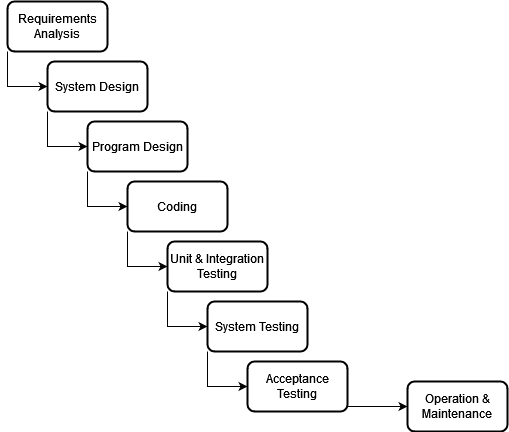
\includegraphics[width=\linewidth]{figures/Waterfall.png}
\end{center}}
{The Waterfall Model of Software Development}
{fig:Waterfall}

Software design can follow a number of different design processes, each with 
their own collection of \sfs{}. A common, traditional approach is the Waterfall 
model (Figure~\ref{fig:Waterfall}) of software 
development~\cite{PfleegerAndAtlee2010Ch2}. 
However, Parnas and Clements~\cite{ParnasAndClements1986} detailed what they 
dubbed a ``rational" design process; an idealized version of software 
development which includes what needs to be documented in corresponding \sfs{}.
The rational design process is not meant to be a linear process like the 
Waterfall model, but instead an iterative process using section stubs for 
information that is not yet available or not fully clear during the time of 
writing. Those stubs are then filled in over the development process, and 
existing documentation is updated so it appears to have been created in a 
linear fashion for ease of review later in the software lifecycle. The rational 
design process involves the following:

\begin{enumerate}
\item Establish/Document Requirements
\item Design and Document the Module Structure
\item Design and Document the Module Interfaces
\item Design and Document the Module Internal Structures
\item Write Programs
\item Maintain
\end{enumerate}

Parnas provided a list of the most important documents~\cite{Parnas2010} 
required for the rational design process, which Smith~\cite{Smith2016} 
\ds{which paper was it?} expanded upon by including complimentary artifacts 
such as source code, verification and validation plans, test cases, and build 
instructions. While there have been many proposed artifacts, the following 
curated list covers those most relevant to this thesis:

\begin{enumerate}
\item System Requirements
\item System Design Document
\item Module Guide
\item Module Interface Specification
\item Program Source Code
\item Verification and Validation Plan
\item Test cases
\item Verification and Validation Report
\item User Manual
\end{enumerate}

This list is not exhaustive of all the types of \sfs{}, as there are many other
design processes which use different types of \sfs{}. Looking at an agile 
approach using Scrum/Kanban, the \sfs{} tend to be distributed in different 
ways. Requirements are documented in tickets under so-called `epics', 
`stories', and `tasks' as opposed to a singular requirements artifact, and the 
acceptance criteria listed on those tickets make up the validation and 
verification plan. 

Regardless of the process used, most attempt to document very similar 
information to that of the rational design process. Using the waterfall model 
as an example, we can see (Table~\ref{tab:RatWatComp}) the rational design 
process and its artifacts map onto the model in a very straightforward manner.

\begin{table}[htbp]
\caption{Comparison of Rational Design Process and Waterfall Model}
\label{tab:RatWatComp}
\begin{tabular}{|p{.25\linewidth}|p{.35\linewidth}|p{.4\linewidth}|}
\hline &&\\
Rational Design phase & Corresponding Waterfall phase(s) & Common \SFS{}
\\&&\\ \hline &&\\
	Establish/ Document Requirements & Requirements Analysis & System 
	Requirements Specification \newline \newline
	Verification and Validation plan
\\&&\\ \hline &&\\
	Design and Document the Module Structure & 
	System Design  & 
	Design Document
\\&&\\ \hline &&\\
	Design and Document the Module Interfaces & 
	Program Design & 
	Module Interface Specification
\\&&\\ \hline &&\\
	Design and Document the Module Internal Structures &
	Program Design &
	Module Guide
\\&&\\ \hline &&\\
	Write Programs & 
	Coding &
	Source code  \newline \newline
	Build instructions
\\&&\\ \hline &&\\
	Maintain & 
	Unit \& Integration Testing \newline \newline System Testing \newline 
	\newline Acceptance 
	Testing \newline \newline Operation \& Maintenance &
	Test cases \newline \newline
	Verification and Validation Report
\\ \hline
\end{tabular}
\end{table}

\SFS{} are important to development in a number of ways, such as easing the 
burden of maintenance and training. We outline the artifacts we are most 
interested below with a brief description of their purpose.

\cardifact{Software Requirements Specification}{Contains the functional and 
nonfunctional requirements detailing what the desired software system should 
do.}
\cardifact{System Design Document}{Explains how the system should be broken 
down and documents implementation-level decisions that have been made for the 
design of the system.}
\cardifact{Module Guide}{In-depth explanation of the modules outlined in the 
System Design Document.}
\cardifact{Module Interface Specification}{Interface specification for each of 
the modules outlined in the System Design Document/Module Guide.}
\cardifact{Program Source Code}{The source code of the implemented software 
system.}
\cardifact{Verification and Validation Plan}{Uses the system requirements to 
document acceptance criteria for each requirement that can be validated.}
\cardifact{Test cases}{Implementation of the Verification and Validation Plan 
in source code (where applicable) or as a step-by-step guide for testers.}
\cardifact{Verification and Validation Report}{Report outlining the results 
after undertaking all of the testing initiatives outlined in the Verification 
and Validation plan and test cases.}

\section{Software Reuse and Software Families}
\subsection{Software/Program Families}
  - Bring up GNU/Linux and different distros as examples of software families
    - (Raspbian v Raspbian lite) = Debian--, etc.
\subsection{Reuse and Reproducible Research}
  - Touch on reuse areas like reproducible research - Gentleman and Lang 2012

Being able to reproduce results, is fundamental to the idea of good science.
When it comes to software projects, there are often many undocumented
assumptions or modifications (including hacks) involved in the finished product.
This can make replication impossible without the help of the original author,
and in some cases reveal errors in the original author's
work~\cite{IonescuAndJansson2013}.

Reproducible research has been used to mean embedding executable code in
research papers to allow readers to reproduce the results
described~\cite{SchulteEtAl2012}.

Combining research reports with relevant code, data, etc.\ is not necessarily
easy, especially when dealing with the publication versions of an author's work.
As such, the idea of \emph{compendia} were
introduced~\cite{GentlemanAndLang2012} to provide a means of encapsulating the
full scope of the work. Compendia allow readers to see computational details, as
well as re-run computations performed by the author. Gentleman and Lang proposed
that compendia should be used for peer review and distribution of scientific
work~\cite{GentlemanAndLang2012}.

Currently, several tools have been developed for reproducible research
including, but not limited to, Sweave~\cite{Leisch2002},
SASweave~\cite{LenthEtAl2007}, Statweave~\cite{Lenth2009},
Scribble~\cite{FlattEtAl2009}, and Org-mode~\cite{SchulteEtAl2012}. The most
popular of those being Sweave~\cite{SchulteEtAl2012}. The aforementioned tools
maintain a focus on code and certain computational details. Sweave,
specifically, allows for embedding code into a document which is run as the
document is being typeset so that up to date results are always included.
However, Sweave (along with many other tools), still maintains a focus on
producing a single, linear document. It is my hope that Drasil will outperform
these existing tools due to its flexibility and its ability to create multiple
artifacts from a knowledge base.

\section{Literate Approaches to Software Development}

There have been several approaches attempting to combine development of program 
code with documentation. Literate Programming and literate software are two 
such approaches that have influenced the direction of this thesis. Each of 
these approaches is outlined in the following sections.

\subsection{Literate Programming}

Literate Programming (LP) is a method for writing software introduced by Knuth 
that focuses on explaining to a human what we want a computer to do rather than 
simply writing a set of instructions for the computer on how to perform the 
task~\cite{Knuth1984}.

Developing literate programs involves breaking algorithms down into
\emph{chunks}~\cite{JohnsonAndJohnson1997} or \emph{sections}~\cite{Knuth1984}
which are small and easily understandable. The chunks are ordered to follow a 
``psychological order''~\cite{PieterseKourieAndBoake2004} if
you will, that promotes understanding. They do not have to be written in the 
same order that a computer would read them. It should also be noted that in a 
literate program, the code and documentation are kept together in one source. 
To extract runnable code, a process known as \emph{tangle} must be performed on 
the source. A similar process known as \emph{weave} is used to extract and 
typeset the documentation.

There are many advantages to LP beyond understandability. As a program is
developed and updated, the documentation surrounding the source code is more 
likely to be updated simultaneously. It has been experimentally found that 
using LP ends up with more consistent documentation and 
code~\cite{ShumAndCook1993}. There are many downsides to having inconsistent 
documentation while developing or maintaining 
code~\cite{Kotula2000,Thimbleby1986}, while the benefits of consistent 
documentation are numerous~\cite{Hyman1990, Kotula2000}. Keeping the advantages 
and disadvantages of good documentation in mind we can see that more effective, 
maintainable code can be produced if properly using 
LP~\cite{PieterseKourieAndBoake2004}.

Regardless of the benefits of LP, it has not been very popular with 
developers~\cite{ShumAndCook1993}. However, there are
several successful examples of LP's use in SC. Two such literate programs that 
come to mind are VNODE-LP~\cite{Nedialkov2006} and ``Physically Based 
Rendering: From Theory to Implementation''~\cite{PharrAndHumphreys2004} a 
literate program and textbook on the subject matter. Shum and 
Cook~\cite{ShumAndCook1993} discuss the main issues behind LP's lack of 
popularity which can be summed up as dependency on a 
particular output language or text processor, and the lack of flexibility on 
what should be presented or suppressed in the output.

There are several other factors which contribute to LP's lack of popularity and 
slow adoption thus far. While LP allows a developer to write their code and its 
documentation simultaneously, that documentation is comprised of a single 
artifact which may not cover the same material as standard artifacts software 
engineers expect (see Section~\ref{sec:sfs} for more details). LP also does not 
simplify the development process: documentation and code are written as usual, 
and there is the additional effort of re-ordering the chunks. The LP 
development process has some benefits such as allowing developers to follow a 
more natural flow in development by writing chunks in whichever order they 
wish, keep the documentation and code updated simultaneously (in theory) 
because of their co-location, and automatically incorporate code chunks into 
the documentation to reduce some information duplication.

There have been many attempts to increase LP's popularity by focusing on 
changing the output language or removing the text processor dependency. Several
new tools such as CWeb (for the C language), DOC++ (for C++), noweb 
(programming language independent), and others were developed. Other tools such 
as javadoc (for Java) and Doxygen (for multiple languages) were also influenced 
by LP, but differ in that they are merely document extraction tools. They do 
not contain the chunking features which allow for re-ordering algorithms.

With new tools came new features including, but not limited to, phantom
abstracting~\cite{ShumAndCook1993}, a ``What You See Is What You Get'' (WYSIWYG)
editor~\cite{FritzsonGunnarssonAndJirstrand2002}, and even movement away from 
the ``one source'' idea~\cite{Simonis2003}.

While LP is still not mainstream~\cite{Ramsey1994}, these more robust 
tools helped drive the understanding behind what exactly LP tools must 
do. In certain domains LP is becoming more standardized, for 
example: Agda, Haskell, and R support LP to some extent, even though it is not 
yet common practice. R has good tool support, with the most popular being
Sweave~\cite{Leisch2002}, however it is designed to dynamically create
up-to-date reports or manuals by running embedded code as opposed to being used
as part of the software development process. 

\subsection{Literate Software}

A combination of LP and Box Structure~\cite{Mills1986} was proposed as a new
method called ``Literate Software Development''
(LSD)~\cite{AlMatiiAndBoujarwah2002}. Box structure can be summarized as the
idea of different views which are abstractions that communicate the same
information in different levels of detail, for different purposes. Box
structures consist of black box, state machine, and clear box structures. The
black box gives an external (user) view of the system and consists of stimuli
and responses; the state machine makes the state data of the system visible (it
defines the data stored between stimuli); and the clear box gives an internal
(designer's) view describing how data are processed, typically referring to
smaller black boxes~\cite{Mills1986}. These three structures can be nested as
many times as necessary to describe a system.

LSD was developed with the intent to overcome the disadvantages of both LP and
box structure. It was intended to overcome LP's inability to specify interfaces
between modules, the inability to decompose boxes and implement the design
created by box structures, as well as the lack of tools to support box
structure~\cite{Deck1996}.

The framework developed for LSD, ``WebBox'', expanded LP and box structures in a
variety of ways. It included new chunk types, the ability to refine chunks, the
ability to specify interfaces and communication between boxes, and the ability
to decompose boxes at any level. However, literate software (and LSD) remains
primarily code-focused with very little support for creating other software
artifacts, in much the same way as LP.

\section{Generative Programming}
 - ?
                  
       \setcounter{figure}{0}
       \setcounter{equation}{0}
       \setcounter{table}{0}

  \chapter{A look under the hood: \\ Our process}

\ds{Make sure we talk about continuous integration / git processes / etc.
Actually might belong in the next chapter - iteration and refinement}

The first step in removing unnecessary redundancy is identifying exactly what
that redundancy is and where it exists. To that end we need to understand what
each of our software artifacts is attempting to communicate, who their audience
is, and what information can be considered boilerplate versus system-specific.
Luckily, we have an excellent starting point thanks to the work of many smart
people - artifact templates.

Lots of work \ds{cite some people who did this} has been done to specify 
exactly what should be documented in a given artifact in an effort for 
standardization. Ironically, this has led to many different `standardized' 
templates. Through the examination of a number of different artifact templates, 
we have concluded they convey roughly the same overall information for a given 
artifact. Most differences are stylistic or related to content 
organization and naming conventions.

Once we understand our artifacts, we take a practical, example-driven approach
to identifying redundancy through the use of existing software system case
studies. For each of these case studies, we start by examining the source code
and existing software artifacts to understand exactly what problem they are
trying to solve. From there, we attempt to distill the system-specific knowledge
and generalize the boilerplate.

\section{A (very) brief introduction to our case study systems}
\ds{**NOTE: ensure each artifact has a 'who' (audience), 'what' (problem 
being solved), and 'how' (specific-knowledge vs boilerplate) - this last one 
may not be necessary}

To simplify the process of identifying redundancies and patterns, we have chosen
several case studies developed using common artifact templates, specifically 
those used by \smithea{} \ds{source?} Also, as mentioned in 
Section~\ref{sec:scope}, we have chosen software systems that follow the 
$`input' \rightarrow `process' \rightarrow `output'$ pattern. These systems 
cover a variety of use cases, to help avoid over-specializing into one 
particular system type. 

The majority of the aforementioned case studies were developed to solve real
problems. The following cards are meant to be used as a high-level reference to 
each case study, providing the general details at a glance. For the specifics 
of each system, all relevant case study artifacts can be found at \ds{Add a 
link here or put in appendices?}.

\card{\gb}
{We need to efficiently and correctly predict whether a glass 
slab can withstand a blast under given conditions.}
{\ds{TODO - Fill in once all examples in the thesis are done}}

\card{\sw}
{Solar water heating systems incorporating phase change 
 material (PCM) use a renewable energy source and provide a novel way of 
 storing energy. A system is needed to investigate the effect of employing PCM
 within a solar water heating tank.}
{\ds{TODO}}

\card{\np}
{Solar water heating systems provide a novel way of 
heating water and storing renewable energy. A system is needed to investigate
the heating of water within a solar water heating tank.}
{\ds{TODO}}

The NoPCM case study was created as a software family member for the SWHS case
study. It was manually written, removing all references to PCM and thus 
remodeling the system.

\card{\sp}
{A slope of geological mass, composed of soil and rock 
 and sometimes water, is subject to the influence of gravity on the mass. 
 This can cause instability in the form of soil or rock movement which can
 be hazardous. A system is needed to evaluate the factor of safety of 
 a slope's slip surface and identify the critical slip surface of the slope, 
 as well as the interslice normal force and shear force along the critical 
 slip surface.}
{\ds{TODO}}

\card{\pr}
{A system is needed to efficiently and correctly predict
 the landing position of a projectile.}
{\ds{TODO}}

The Projectile case study, was the first example of a system 
created solely in Drasil, i.e. we did not have a manually created version to 
compare and contrast with through development. As such, it will not be 
referenced often until \ds{DRASILSECTION} since it did not inform Drasil's 
design or development until much further in our process. The Projectile case 
study was created post-facto to provide a simple, understandable example for a 
general audience as it requires, at most, a high-school level understanding of 
physics. 

\card{\gp}
{Many video games need physics libraries that simulate 
 objects acting under various physical conditions, while simultaneously being 
 fast and efficient enough to work in soft real-time during the game. 
 Developing a physics library from scratch takes a long period of time and is 
 very costly, presenting barriers of entry which make it difficult for game 
 developers to include physics in their products.}
{\ds{TODO}}

After carefully selecting our case studies, we went about a practical approach
to find and remove redundancies. The first step was to break down each artifact
type and understand exactly what they are trying to convey.


\section{Breaking down \sfs}
\label{sec:breakdown}

As noted earlier, for our approach to work we must understand exactly what each
of our artifacts are trying to say and to whom.\footnote{Refer to 
Section~\ref{sec:sfs} for a general summary of \sfs{}.} By selecting our case 
studies from those developed using common artifact templates, we have given 
ourselves a head start on that process, however, there is still much work to be 
done.

The following subsections present a brief sampling of our process of breaking 
down \sfs{}, acknowledging that a comprehensive overview would be excessively 
lengthy.

\subsection{SRS}
\label{sec:breakdown:srs}

To start, we look at the Software Requirements Specification (SRS). The SRS
(or some incarnation of it) is one of the most important artifacts for any
software project as it specifies what problem the software is trying to solve.
There are many ways to state this problem, and the template from \smithea{} has 
given us a strong starting point. Figure~\ref{fig:SRSToC} shows the table of 
contents for an SRS using the \smithea{} template.

\fig{
  \begin{center}
\footnotesize
\begin{enumerate}[nosep, label*=\arabic*.]
\item Reference Material
\begin{enumerate}[nosep, label*=\arabic*.]
  \item Table of Units
  \item Table of Symbols
  \item Abbreviations and Acronyms
\end{enumerate}
\item Introduction
\begin{enumerate}[nosep, label*=\arabic*.]
  \item Purpose of Document
  \item Scope of Requirements
  \item Characteristics of Intended Reader
  \item Organization of Document
\end{enumerate}
\item Stakeholders
\begin{enumerate}[nosep, label*=\arabic*.]
  \item The Customer
  \item The Client
\end{enumerate}
\item General System Description
\begin{enumerate}[nosep, label*=\arabic*.]
  \item System Context
  \item User Characteristics
  \item System Constraints
\end{enumerate}
\item Specific System Description
\begin{enumerate}[nosep, label*=\arabic*.]
  \item Problem Description
\begin{enumerate}[nosep, label*=\arabic*.]
    \item Physical System Description
    \item Goal Statements
\end{enumerate}
  \item Solution Characteristics Specification
\begin{enumerate}[nosep, label*=\arabic*.]
    \item Assumptions
    \item Theoretical Models
    \item General Definitions
    \item Data Definitions
    \item Instance Models
    \item Data Constraints
    \item Properties of a Correct Solution
\end{enumerate}
\end{enumerate}
\item Requirements
\begin{enumerate}[nosep, label*=\arabic*.]
  \item Functional Requirements
  \item Non-Functional Requirements         
\end{enumerate}
\item Likely Changes
\item Unlikely Changes
\item Traceability Matrices and Graphs
\item Values of Auxiliary Constants
\item References
\item Appendix
\end{enumerate}
  \end{center}
}{The Table of Contents from the (\ds{expanded?}) \smithea{} 
template}{fig:SRSToC}

With the structure of the document in mind, let us look at several of our case
studies' SRS documents to get a deeper understanding of what each section truly
represents. Figure~\ref{fig:csRefSecs} shows the reference section of the SRS 
for \gb. Each of the case studies' SRS contains a similar section so for 
brevity we will omit the others here, but they can be found at \ds{TODO}. 
% Provide a link / ref to relevant appendix
We will look into the case studies in more detail later \ds{will we actually? 
depends on length of chapter}, for now we will try to 
ignore any superficial differences (spelling, grammar, phrasing, etc.) in each 
of them while we look for commonality. We are also trying to determine how the 
non-superficial differences relate to the document template, general problem 
domain, and specific system information.

\fig{
\centering
%\emph{Figure showing the Ref Section of one case 
%			study, split into multiple subfigures - case study TBD}
\begin{subfigure}{\textwidth}
\centering
\fbox{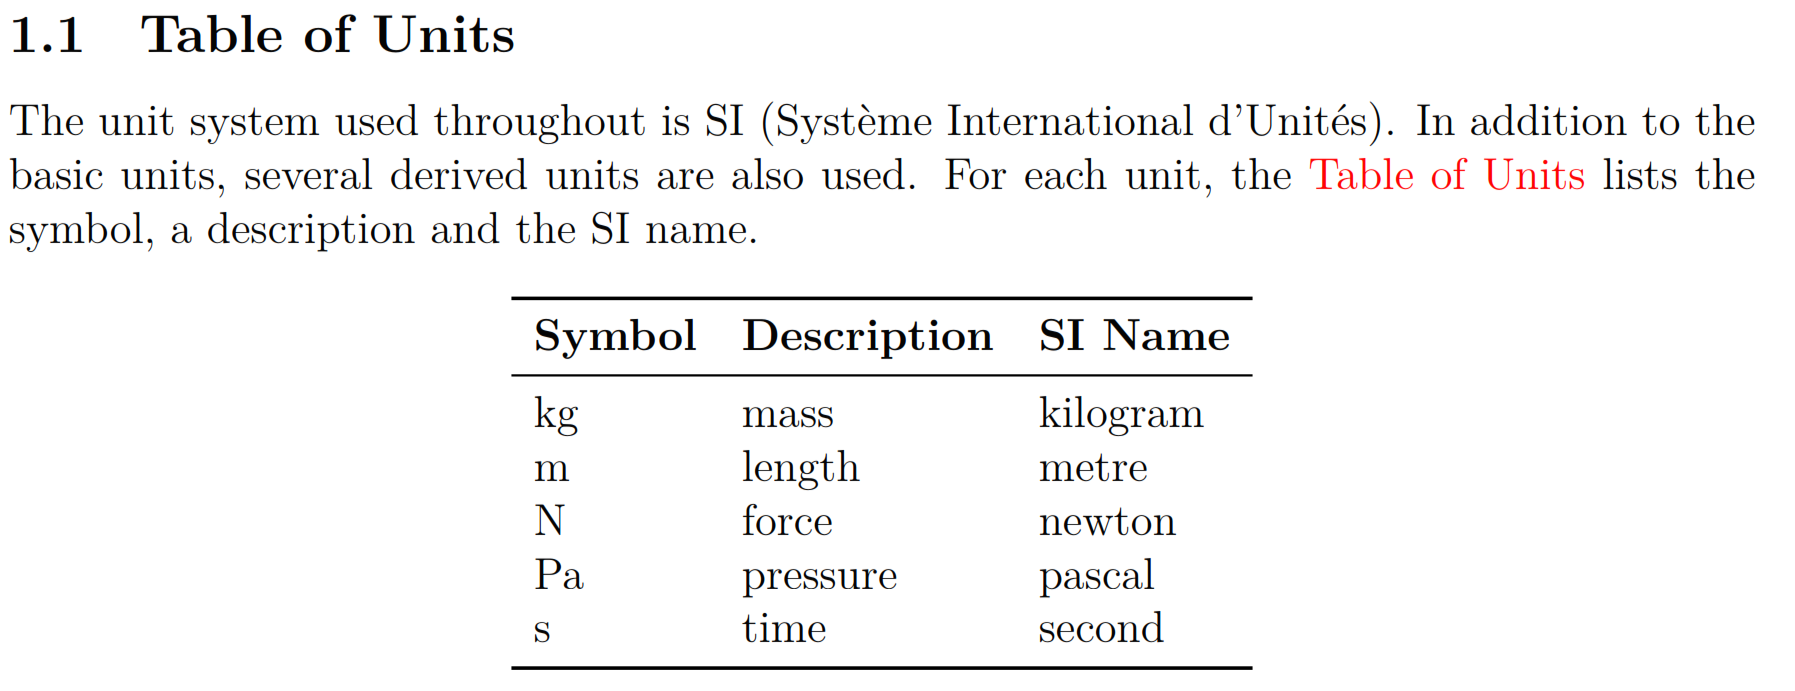
\includegraphics[width=\textwidth]{figures/gb_SRS_ToU.png}}
\caption{Table of Units Section}
\label{fig:gbrtou}
\end{subfigure}

\end{figure}

\begin{figure}\ContinuedFloat

\begin{subfigure}{\textwidth}
\centering
\fbox{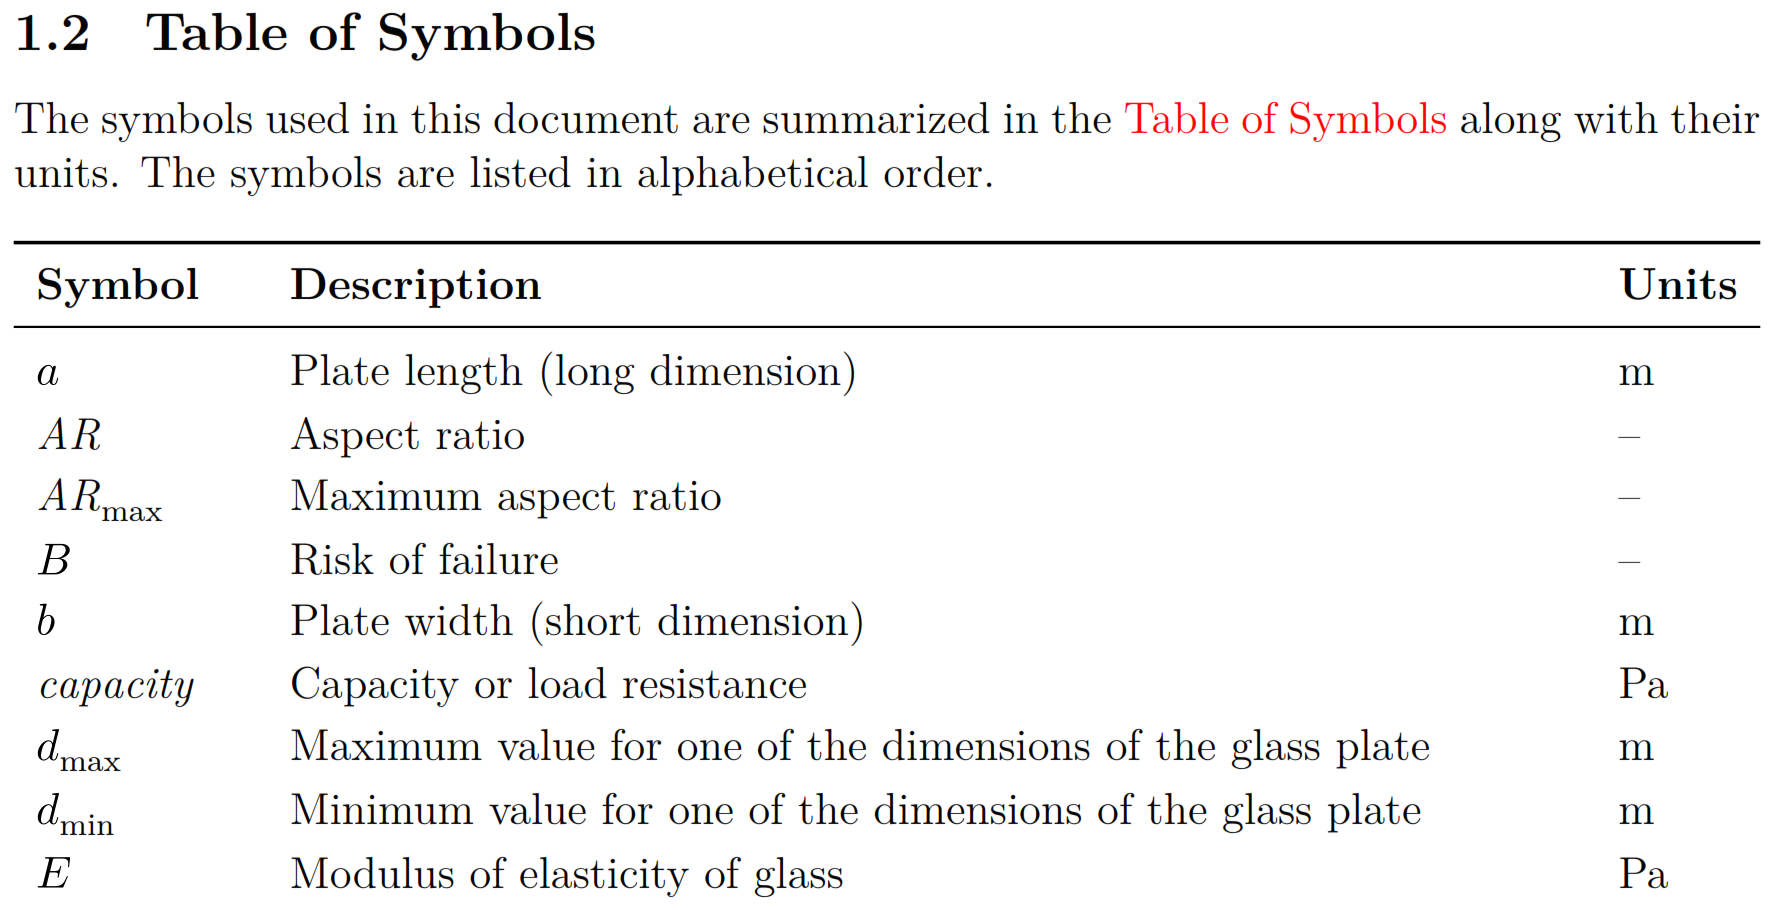
\includegraphics[width=\textwidth]{figures/gb_SRS_ToS.png}}
\caption{Table of Symbols (truncated) Section}
\label{fig:gbrtos}
\end{subfigure}


\begin{subfigure}{\textwidth}
\centering
\fbox{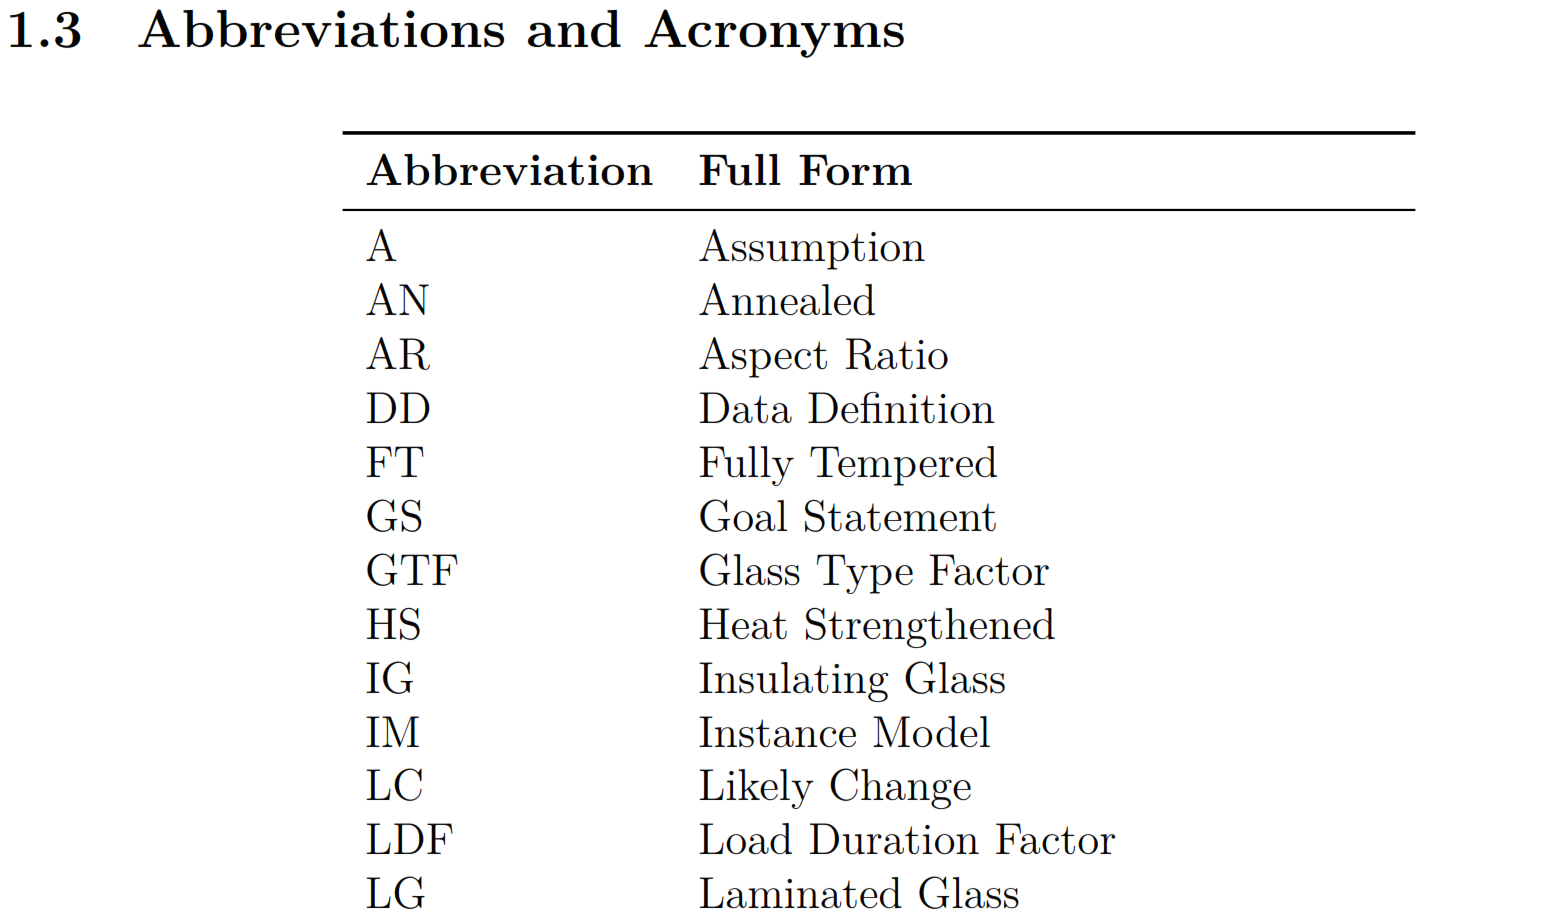
\includegraphics[width=\textwidth]{figures/gb_SRS_ToAA.png}}
\caption{Table of Abbreviations and Acronyms (truncated) Section}
\label{fig:gbrtoa}
\end{subfigure}
}
{The reference sections of \gb}
{fig:csRefSecs}

Looking at the (truncated for space) Table of Symbols, Table of Units, and 
Table of Abbreviations and Acronyms sections (Figure~\ref{fig:csRefSecs}) we 
can see that, barring the table values themselves, they are almost identical. 
The Table of Symbols is simply a table of values, akin to a glossary, specific 
to the symbols that appear throughout the rest of the document. For each of 
those symbols, we see the symbol itself, a brief description of what that 
symbol represents, and the units it is measured in, if applicable. Similarly, 
the Table of Units lists the Syst\`eme International d'Unit\'es (SI) Units used 
throughout the document, their descriptions, and the SI name. Finally, the 
table of Abbreviations and Acronyms lists the abbreviations and their full 
forms, which are essentially the symbols and their descriptions for each of the 
abbreviations.

While the reference material section should be fairly self-explanatory as to 
what it contains, other sections and subsections may not be so clear from their 
name alone. For example, it may not be clear offhand of what constitutes a 
theoretical model compared to a data definition or an instance model. One may 
argue that the author of the SRS, particularly if they chose to use the 
\smithea{} template, would need to understand that difference. However, it is 
not clear whether the intended audience would also have such an understanding. 
Who is that audience? Refer to Section~\ref{sec:sfs}, for more details. A brief 
summary is available in Table~\ref{tab:sfsummary}.

Returning to our exercise of breaking down each section of the SRS to determine 
the subtleties of \emph{what} is contained therein\footnote{The breakdown 
details are omitted for brevity and due to their monotonous nature, although 
the overall process is very much akin to the breakdown of the Reference 
Material section.} it should be unsurprising that each section maps to the 
definition provided in the \smithea{} template. However, as noted above, we can 
see distinct differences in the types of information contained in each section. 
Again we find some is boilerplate text meant to give a generic 
(non-system-specific) overview, some is specific to the proposed system, and 
some is in-between: it is specific to the problem domain for the proposed 
system, but not necessarily specific to the system itself.

Observing the contents of an SRS template adhere to said template may seem 
mundane, but it is a necessary step before we can move on to other \sfs{}. 
Without understanding what the SRS template intends to convey it is hard to 
assess weather or not the case study SRS conveys that information. With that in 
mind, we can move on to the MG and source code.

\ds{Current plan for following subsections: Brief description of the \sf{}, 
show an example of similarities within (ex. MG/MIS have a section per module, 
each section is organized the same way, some are filled in, some aren't), then 
follow a requirement through the MG to something in the MIS and finally to 
code. We'll dissect differences between case studies when looking at the 
patterns in Section~\ref{sec:patterns}. This also plants the seeds of "see, 
there's the same info moving from SRS $\rightarrow$ MG $\rightarrow$ MIS** 
$\rightarrow$ Code without stating it 
explicitly, which we can then do in the pattern section.}

\ds{Example to use should be a DD/IM from GlassBR, goes to calculations module 
in the MG, and finally a method in the source code}

\subsection{Module Guide}
\label{sec:breakdown:mg}

The module guide (MG) is a \sf{} that details the architecture of a given 
software system. It holds a number of design decisions around sensibly grouping 
functionalities within the system into modules to fulfill the requirements laid 
out in the SRS. For example, one might have an input/output module for handling 
user input and giving the user feedback through the display (ie. via print 
commands or some other output), or a calculations module that contains all of 
the calculation functions being performed in the normal operation of the given 
software system. The \smithea{} MG template also includes a traceability matrix 
for ease of verifying which requirements are fulfilled by which modules. 
Finally, the MG includes considerations for anticipated or unlikely changes 
that the system may undergo during its lifecycle.

\fig{
\begin{center}
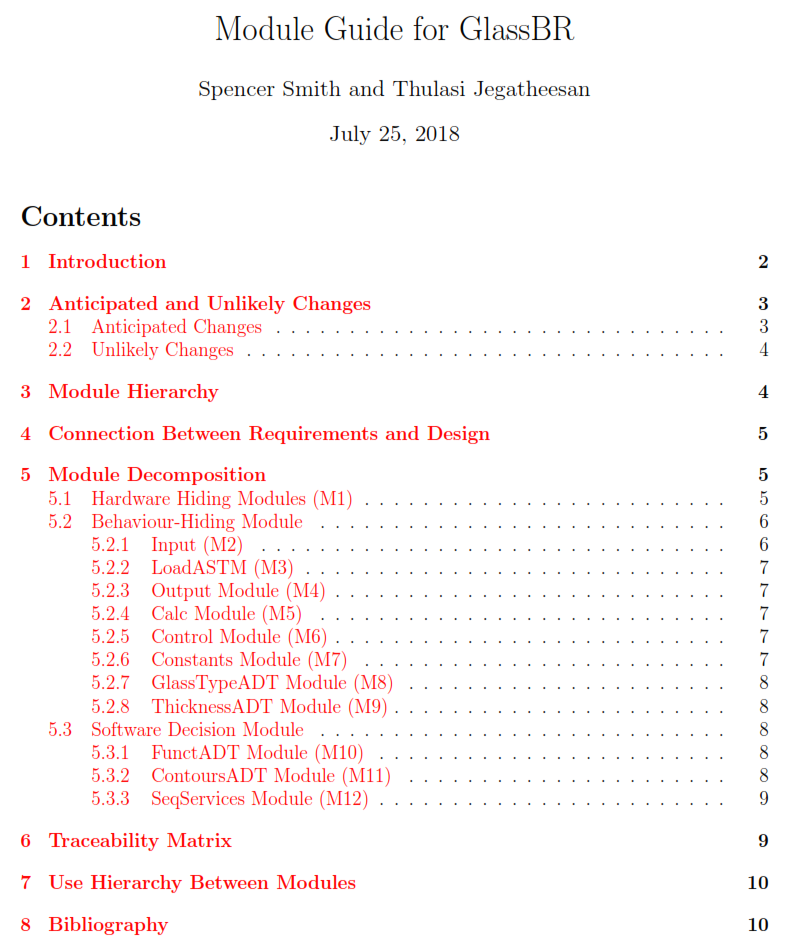
\includegraphics[width=\linewidth]{figures/gb_MG_ToC.png}
\end{center}}
{Table of Contents for GlassBR Module Guide}
{fig:gbrmgtoc}

Figure~\ref{fig:gbrmgtoc} shows the table of contents for the \gb{} case 
study's MG. For the sake of brevity we will omit the other case studies 
here (they can be found at \ds{TODO}). Just as with the SRS we are looking for 
commonality and understanding of what the document is trying to portray to the 
reader. As such we will ignore superficial differences between the MG sections. 
As the MG is a fairly short document we will look at each of the most relevant 
sections as part of this exercise.

Breaking down the MG by section, we can see that the introduction is itself 
completely generic boilerplate explaining the purpose of the MG, the audience, 
and some references to other works that explain why we would make certain 
choices over other (reasonable) ones given the opportunity. There is nothing 
system-specific, nor specific to the given problem domain of the case study.

Following through the table of contents into the ``Anticipated and Unlikely 
Changes" section, we see that again the introductions to this section and 
its subsections are generic boilerplate, however the details of each section 
are not. Both subsections are written in the same way: as a list of labeled 
changes (AC\# for anticipated change, UC\# for unlikely change). This is the 
first place we see both problem-domain and system-specific information 
Interestingly, the Module Hierarchy section follows the same general style: it 
is a list of modules which represent the leaves of the module hierarchy tree 
and each one is labeled (M\#).

\fig{
\begin{center}
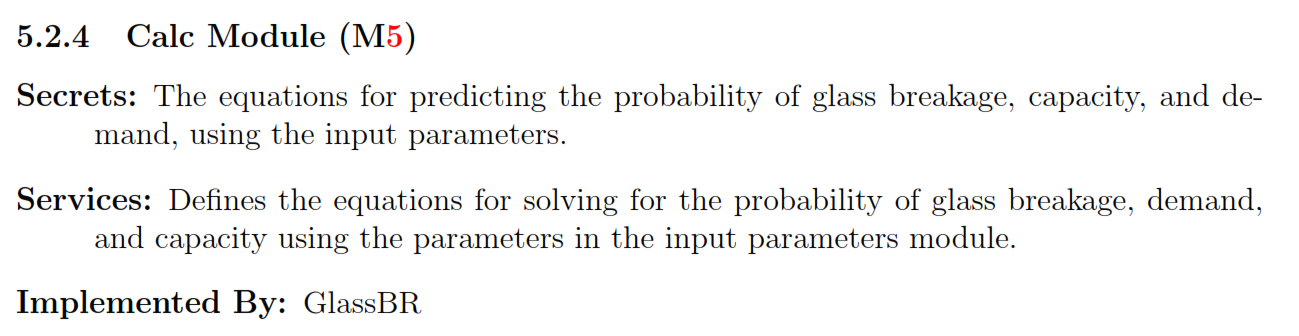
\includegraphics[width=\linewidth]{figures/gb_MG_CM.png}
\end{center}}
{Calc Module from the \gb{} Module Guide}
{fig:gbrmgcm}

Skipping ahead to the module decomposition, we find a section heading for each 
Level 1 module in the hierarchy, followed by subsections describing the Level 2 
modules. The former are almost entirely generic boilerplate (for example common 
Level 1 modules include: Hardware-Hiding, Behaviour-Hiding, and 
Software Decision modules), but the latter are problem-domain or system 
specific. An example of a system-specific module is shown in 
Figure~\ref{fig:gbrmgcm}. 

Each module is described by its secrets, services, and what it will be 
implemented by. For example, a given module could be implemented by the 
operating system (OS), the system being described (ex. \gb{}), or a third party 
system/library that will inter-operate with the given system.

Finally we have a traceability matrix and use hierarchy diagram. Both are 
visual representations of how the different modules implement the requirements 
and use each other respectively. The traceability matrix provides a direct and 
obvious link between the SRS and MG, where other connections between the two 
\sfs{} have been implicit until this point. Generally, the next \sf{} would be 
the MIS, however as it is structured so similarly to the MG (one section per 
module, each section organized in a very similar way, a repeated use hierarchy, 
etc) we will skip it for brevity. The MIS includes novel system-specific, 
implementation-level information denoting the interfaces between modules, but 
for our current exercise does not provide any revelations beyond that of the MG.

The MG gives us a very clear picture of \textit{decisions} made by the system 
designers, as opposed to the knowledge of the system domain, problem being 
solved, and requirements of an acceptable solution provided in the SRS. The MG 
provides platform and implementation-specific decisions, which will eventually 
be translated into implementation details in the source code. With that in 
mind, let us move on to the source code.

\subsection{Source Code}
\label{sec:breakdown:code}

The source code is arguably the most important \sf{} in any given software 
system since it serves as the set of instructions that a computer executes in 
order to solve the given problem. With only the other \sfs{} and without the 
source code, we would have a very well defined problem and acceptance criteria 
for a possible solution, but would never actually solve the problem.

\fig{
\begin{center}

\begin{forest}
  for tree={
    font=\ttfamily,
    grow'=0,
    child anchor=west,
    parent anchor=south,
    anchor=west,
    calign=first,
    edge path={
      \noexpand\path [draw, \forestoption{edge}]
      (!u.south west) +(7.5pt,0) |- node[fill,inner sep=1.25pt] {} (.child 
      anchor)\forestoption{edge label};
    },
    before typesetting nodes={
      if n=1
        {insert before={[,phantom]}}
        {}
    },
    fit=band,
    before computing xy={l=25pt},
  }
[/src/Python
  [Calc.py]
  [Constants.py]
  [ContoursADT.py]
  [Control.py]
  [Exceptions.py]
  [FunctADT.py]
  [GlassTypeADT.py]
  [Input.py]
  [LoadASTM.py]
  [Output.py]
  [SeqServices.py]
  [ThicknessADT.py]
]
\end{forest}

\end{center}
}
{Python source code directory structure for \gb{}}
{fig:gbsrcstruct}

As the source code is the executable set of instructions, one would expect it 
to be almost entirely system and problem-domain specific with very little 
boilerplate. Looking into the source of our case studies, we find this to be 
mostly true barring the most generic of library use (ex. 
\code{C}{stdio} in C).

Returning to our example of the MG from \gb{} (Figure~\ref{fig:gbrmgtoc}) and 
comparing it to the python source code structure shown in 
Figure~\ref{fig:gbsrcstruct} we can see that the source code follows almost 
identically in structure to the module decomposition. The only difference being 
the existence of an exceptions module defining the different types of
exceptions that may be thrown by the other modules. While this can be 
considered a fairly trivial difference, likely made for ease of maintenance, 
readability, and extensibility, it highlights that the two \sfs{} are out of 
sync. We speculate this difference was caused by a change made during the 
implementation phase, wherein the MG was not updated to reflect the addition of 
an exceptions module.

\fig{
\lstinputlisting[language=Python, firstline=5, 
lastline=61, firstnumber=5]{code/Calc.py}
}{Source code of the Calc.py module for \gb{}}{fig:gbrsrccalc}

Let us look deeper into the code for one specific module, for example the Calc 
module introduced in the MG~(Figure~\ref{fig:gbrmgcm}). The source code for 
said module can be found in Figure~\ref{fig:gbrsrccalc}. In the source code we 
see a number of calculation functions, including those that calculate the 
probability of glass breakage, demand (also known as \emph{load} or $q$), and 
capacity (also known as \emph{load resistance} or $LR$) as outlined in the 
\emph{secrets} section of the Calc module definition in the MG. We also see a 
number of intermediary calculation functions required to calculate these values 
(for example \code{python}|calc_NFL| and its dependencies).

The source code provides clear instructions to the machine on how to calculate 
each of these values and their intermediaries; it provides the actionable steps 
to solve the given problem. When we compare the code with relevant sections of 
the SRS, specifically the Data Definitions (DDs) for each term, we can see a 
very obvious transformation from one form to the other; the symbol used by the 
DD is the (partial) name of the function in the source code and the equation 
from the DD is calculated within the source code. This is one of many patterns 
we see across our \sfs{} within each case study.

\section{Identifying Repetitive Redundancy}
\label{sec:patterns}

From the examples in Section~\ref{sec:breakdown}, we can see a number of simple 
patterns emerging with respect to organization and information repetition 
within a case study. Upon applying our process to all of the case studies and 
adopting a broader perspective, numerous instances emerge where patterns 
transcend individual case studies and remain universally applicable. Several of 
these patterns should be unsurprising, as they relate to the template of a 
particular \sf{}. It is interesting, however, that patterns of information 
organization crop up within a given \sf{} in multiple places, containing 
distinct information.

Returning to our example from Section~\ref{sec:breakdown:srs}, looking only at 
the reference section of our SRS template, we have already found three 
subsections that contain the majority of their information in the same 
organizational structure: a table defining terms with respect to their symbolic 
representation and general information relevant to those terms. Additionally, 
we can see that the Table of Units and Table of Symbols have an introductory 
blurb preceding the tables themselves, whereas the Table of Abbreviations and 
Acronyms does not. Inspecting across case studies, we observe that the 
introduction to the Table of Units is nothing more than boilerplate text 
dropped into each case study verbatim; it is completely generic and applicable 
to \emph{any} software system using SI units. The introduction to the Table of 
Symbols also appears to be boilerplate across several examples, however, it 
does have minor variations which we can see by comparing 
Figure~\ref{fig:gbrtos} to Figure~\ref{fig:gptos} (\gb{} compared to \gp{}). 
These variations reveal the obvious: the variability between systems is greater 
than simply a difference in choice of symbols, and so there is some 
system-specific knowledge being encoded. While we can intuitively infer this 
conclusion based solely on each system addressing a different problem, our 
observation of the (structural) patterns within this SRS section confirms it.

\fig{
\centering
\fbox{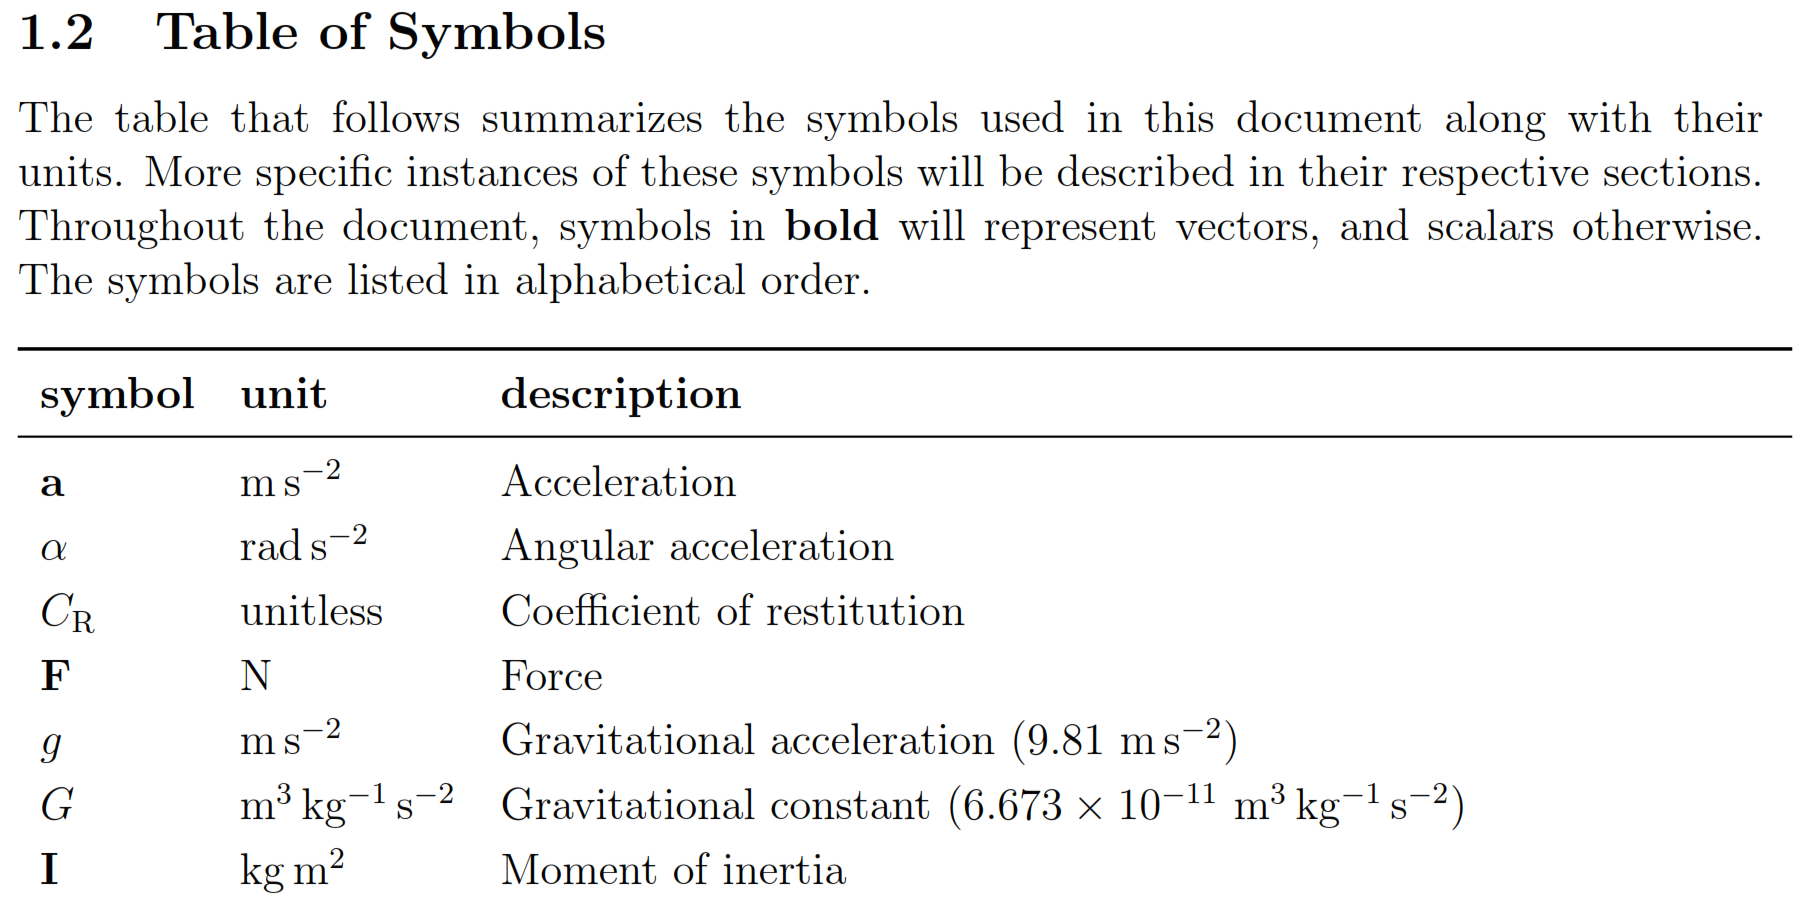
\includegraphics[width=\textwidth]{figures/gp_SRS_ToS.png}}
}
{Table of Symbols (truncated) Section from \gp{}}
{fig:gptos}

The reference section of the SRS provides a lot of knowledge in a very 
straightforward and organized manner. The basic units provided in the table of 
units give a prime example of fundamental, global knowledge shared across 
domains. Nearly any system involving physical quantities will use one or more 
of these units. On the other hand, the table of symbols provides 
system/problem-domain specific knowledge that will not be useful across 
unrelated domains. For example, the stress distribution factor $J$ from GlassBR 
may appear in several related problems, but would be unlikely to be seen in 
something like SWHS, NoPCM, or Projectile. Finally, acronyms are very 
context-dependent. They are often specific to a given domain and, without a 
coinciding definition, it can be very difficult for even the target audience to 
understand what they refer to. Within one domain, there may be several acronyms 
that look identical, but mean different things, for example: PM can refer to a 
Product Manager, Project Manager, Program Manager, Portfolio Manager, etc.

By continuing to breakdown the SRS and other \sfs{}, we are able to find many 
more patterns of knowledge repetition. For example, we see the same concept 
being introduced in multiple areas within a single artifact and across 
artifacts in a project.
\fig{
\centering
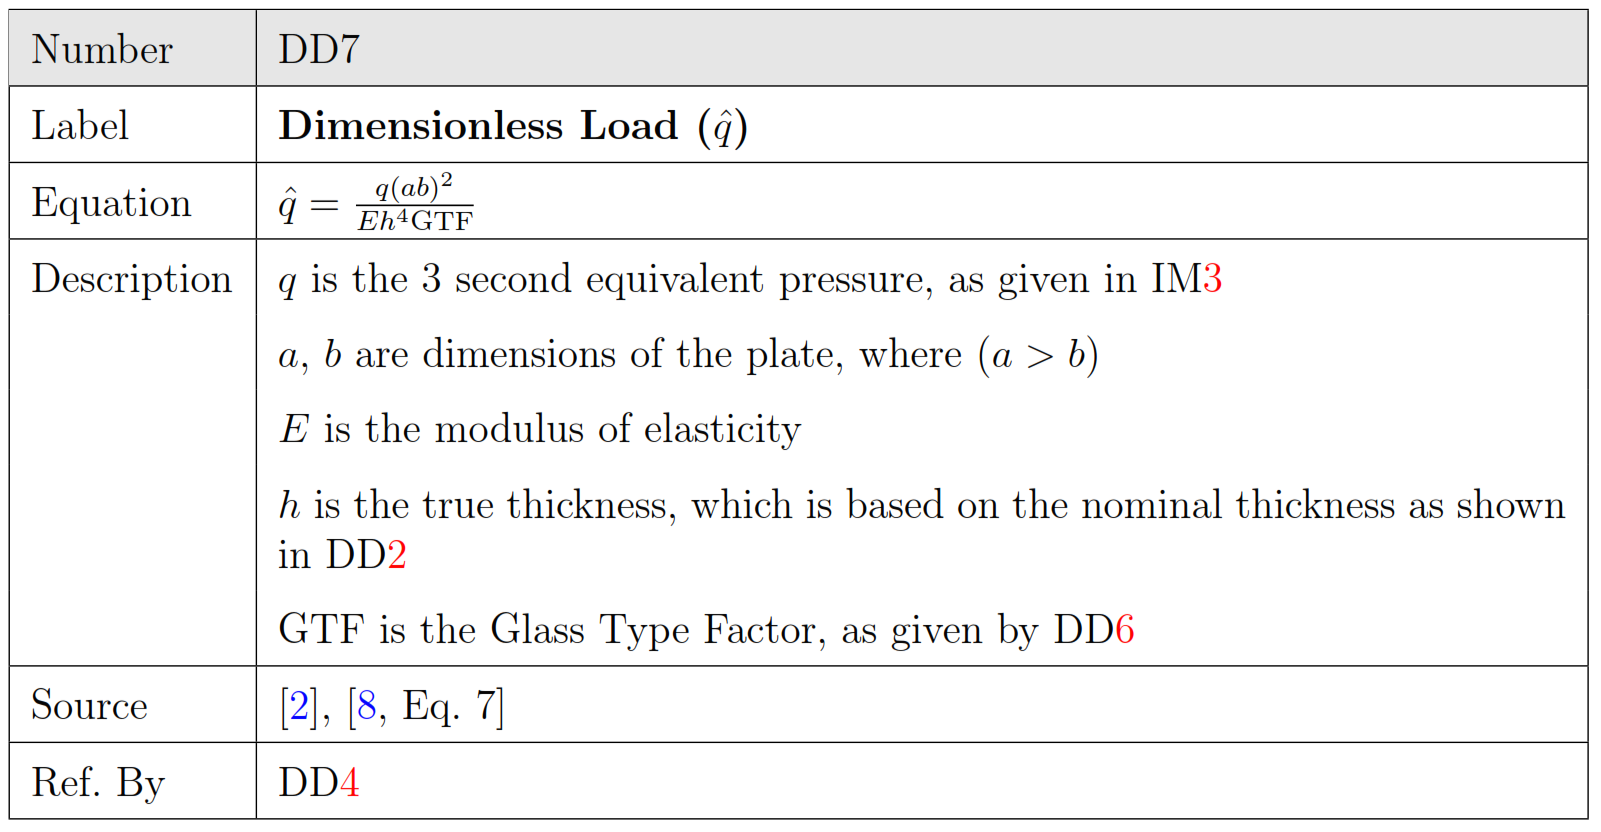
\includegraphics[width=\textwidth]{figures/gb_dd_q.png}}
{Data Definition for Dimensionless Load ($\hat{q}$) from \gb{} SRS}
{fig:gbrddq}
Figure~\ref{fig:gbrddq} shows the data definition for $\hat{q}$ in \gb{}. That 
same term was previously defined with fewer details in the table of symbols 
(omitted here for brevity), as well as showing up implicitly or in passing 
in the MG (Figure~\ref{fig:gbrmgcm} and the \emph{loadASTM} module 
respectively), and implemented in the Source Code (Figure~\ref{fig:gbrsrccalc} 
lines 11-14). It should be noted that the SRS contains many references to 
$\hat{q}$, such as in the data definitions of the Stress Distribution Factor 
($J$) and Non-Factored Load ($NFL$). There are also implied references through 
intermediate calculations, for example the Calculation of Capacity ($LR$) is 
defined in terms of $NFL$ which relies on $\hat{q}$.

Although the full definition of $\hat{q}$ is initially provided 
for a human audience only once, it is necessary to reference it in different 
ways for different audiences. Each audience is expected to grasp the symbol's 
meaning within their given context or consult other \sfs{} for more 
comprehensive understanding. When reading the SRS, the data definitions and 
other reference materials play a crucial role in swiftly comprehending the 
complete definition of $\hat{q}$ in relation to the system's inputs, outputs, 
functional requirements, and acceptance criteria.

The MG, on the other hand, briefly mentions $\hat{q}$ when defining the 
responsibilities of both the \emph{loadASTM} and \emph{Calc} modules (the 
former being responsible for loading values from a file, and the latter 
utilizing those values for calculations), whereas the source code provides a 
highly detailed definition to ensure accurate execution of the relevant 
calculation(s).

The varying level of detail across the \sfs{} should not come as a surprise 
since each \sf{} targets a different audience and their specific needs at 
various stages of the software development process. Although the level of 
verbosity may differ, the core information remains consistent: the authors are 
consistently referring to the definition of $\hat{q}$ via its symbolic 
representation, regardless of the level of detail incorporated. The goal is to 
convey relevant aspects of knowledge of a given term, while eliding that which 
is deemed superfluous, based on the context and the specific requirements of 
our audience. In other words, the authors only \emph{project} some portion of 
their knowledge of given terms at a given time, depending on their needs 
(precision, brevity, clarity, etc.), the expectations of the audience, and 
contextual relevance. \footnote{We have only referred to the term as $\hat{q}$ 
in this section to emphasize our argument and make a meta-argument that the 
definition is irrelevant to our audience in this example. What matters is the 
symbolic reference, which we share a common understanding of.} The audience, on 
the other hand, engages in \emph{knowledge transformation}, whereby they 
consume the representation (projected knowledge) and transform it into their 
own internal representation, based on their personal knowledge-base.

Relying on common representations, eliding definitions, projecting and 
transforming knowledge are fundamental to the way humans communicate. They are 
readily observable in all forms of communications, whether written or oral, as 
we assign meaning to given sounds and symbols (words) according to the agreed 
upon grammar of a given language and use those words (knowledge projections) to 
simplify communication to a given audience. A context-specific glossary, or 
more generally a dictionary, is a prime example of a knowledge-base that we use 
for communication via knowledge projections and transformations. By maintaining 
a shared vocabulary, we can communicate using the symbolic representations 
(words) instead of requiring terms to be decomposed (defined) to their most 
basic form. However, communication of this sort is still imperfect, due to gaps 
in shared knowledge between participants or misunderstanding of overloaded 
terms. Interpersonal communications can involve nuance and context-dependent 
interpretations, yet they still boil down to knowledge projection on the part of
the communicator and knowledge transformation on the part of the communicatee.
The latter can infer context, or be provided with explicit context, which 
affirms their use of the appropriate knowledge transformations.

Returning to the context of software systems, if we broaden our view from a 
single system, to a software family, we can also find patterns of commonality 
and repeated knowledge across the various \sfs{} of the family members (For 
example the SWHS and NoPCM case studies) as they have been developed to solve 
similar, or in our case nearly identical, problems. Software family members are 
good examples to help determine what types of information or knowledge provided 
in the \sfs{} belong to the system-domain, problem-domain, or are simply 
general (boilerplate).

\fig{
\centering
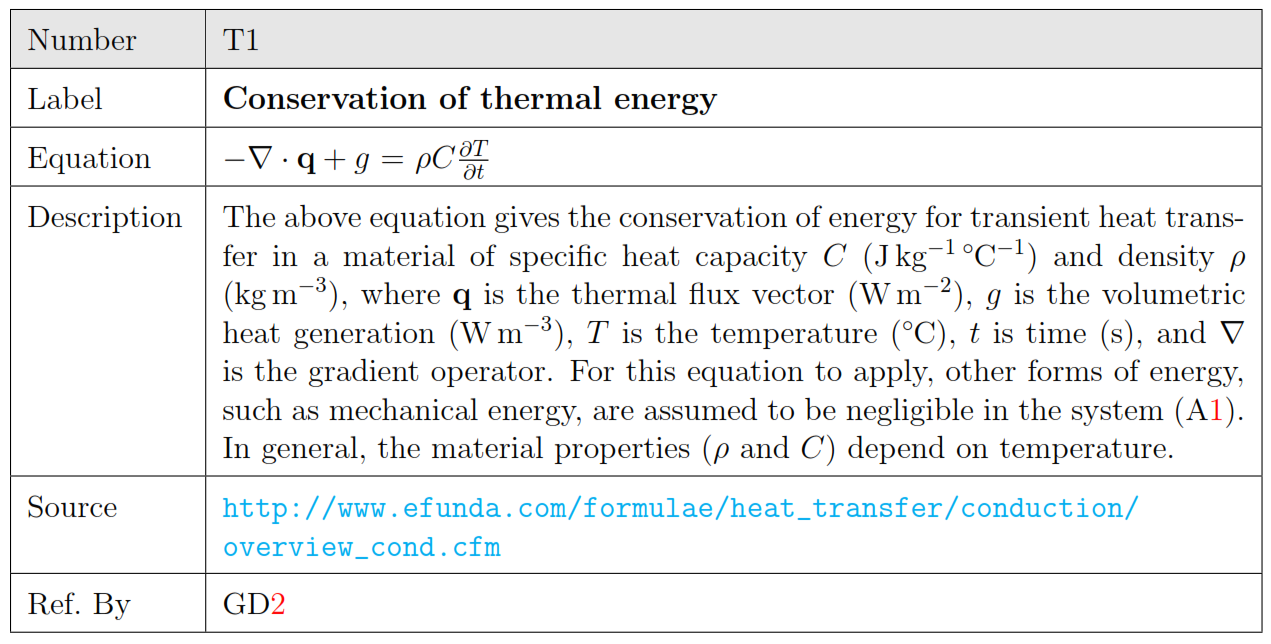
\includegraphics[width=\textwidth]{figures/swhs_TM1.png}}
{Theoretical Model of conservation of thermal energy found in both the SWHS and 
NoPCM SRS}
{fig:swhstm1}

Looking at SWHS and NoPCM, we can easily find identical theoretical models 
(TMs) as the underlying theory for each system is based on the problem domain 
(see example in Figure~\ref{fig:swhstm1}).
However, when we follow the derivations from the TMs to the Instance Models 
(IMs), we find the resulting equations have changed due to the context of the 
system; the lack of PCM has changed the relevant equations for calculating the 
energy balance on water in the tank as shown in Figure~\ref{fig:swhsnopcmim1}.

\fig{
\centering
%\emph{Figure showing the Ref Section of one case 
%			study, split into multiple subfigures - case study TBD}
\begin{subfigure}{\textwidth}
\centering
\fbox{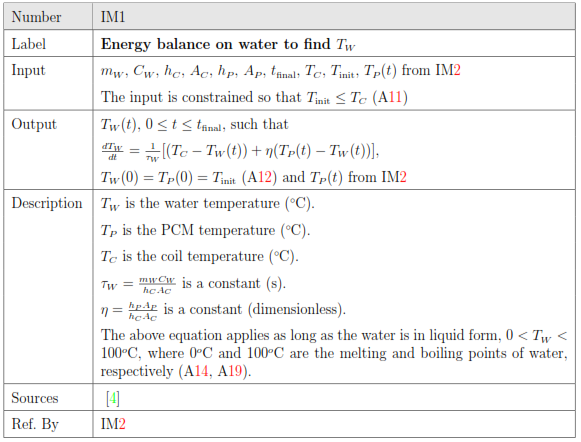
\includegraphics[width=0.8\textwidth]{figures/swhs_IM1.png}}
\caption{SWHS Instance Model for Energy Balance on Water}
\label{fig:swhs_im1}
\end{subfigure}
\begin{subfigure}{\textwidth}
\centering
\fbox{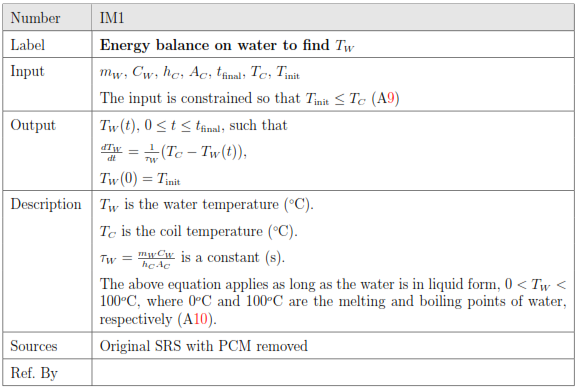
\includegraphics[width=0.8\textwidth]{figures/nopcm_IM1.png}}
\caption{NoPCM Instance Model for Energy Balance on Water}
\label{fig:nopcm_im1}
\end{subfigure}
}
{Instance Model difference between SWHS and NoPCM }
{fig:swhsnopcmim1}

While the above examples are fairly small and specific, they are indicative of 
a larger, more generalizable, set of patterns of knowledge organization and 
repetition. These patterns are at their core: the use of common knowledge that 
has been projected through some means, and patterns of organization of those 
knowledge projections within \sfs{}. Common knowledge, in this case, refers to 
one of three categories of knowledge: system-specific, domain-specific, or 
common to \sfs{} as a whole. It should also be noted that knowledge projections 
may include the identity projection (ie. the full, unabridged definition) as 
they are dependent on the relevance to the audience of the given \sf{}. 
Regardless, the captured knowledge fundamentally underlies these patterns of 
repetition, and is where we need to focus if we intend to reduce unnecessary 
redundancy.

\section{Organizing knowledge - a fluid approach}
%  **Subsec roadmap:
%    - We see the patterns above, we can generalize a lot of that
%    - Direct repetition (copy-paste) vs indirect repetition (view-changes)
%    require us to pull together knowledge from all artifacts into one place
%    - Some can be derived automatically, the rest must be explicitly stated
%    - We need to create a categorization system (hint at chunks) that is both
%    robust and extensible to cover a wide variety of use cases.
%    - Finally the templates give us structure
%
%  **NOTE: Under the hood section should explain the process of how we 
%determined
%  what we needed to do. What we ended up doing should come in the following
%  section(s) - no 'real' implementation details, only conceptual stuff here.
%
%- Some ``boilerplate" information is actually in the domain of \sf{} writing 
%and 
%thus is so broad, yet relevant to everything we do, that we consider it 
%completely general. Things like stakeholders, characteristics of the intended 
%audience, etc.

Given the knowledge categories and patterns of use across \sfs{} we have seen 
in the previous section, we can generalize knowledge projections by their 
projection functions. \ds{What follows is very rough and may need some 
definitions/tweaking to be more clear, but it makes sense in my head} Identity 
projection functions directly repeat knowledge 
verbatim i.e. $p(K) \equiv K$ for some piece of knowledge $k$ \ds{I think I'll 
remove all of the set notation here, it comes out of nowhere and probably won't 
come up anywhere else or be defined anywhere so it's a bit jarring. I'm leaving 
it in for now because it makes sense to me}. For example a 
copy-and-paste approach would be an identity projection.  It should be noted in 
our case that as long as the projection used contains the full definition and 
context of a piece of knowledge, that projection is considered an identity 
projection regardless of changes to notation (ex. ``$x = y$" vs ``$y = x$") or 
language (ex. ``$x = y$" vs ``$x$ is equal to $y$" vs ``x est \'egal \`a y"). 
\ds{Please correct my French if I'm wrong here}
Non-identity projections require using representations that elide some details 
of the knowledge at hand to make it more palatable for the audience of the 
given \sf{} i.e. $p(K) \subset K$. Similarly, we can have multivariant 
projection functions (whether identity or not) which project knowledge from 
several places into one form, i.e. $p(K,L,M) \subseteq K\cup L\cup M$.

In both cases, we have a knowledge core that is fully defined and then we apply 
a projection function to retrieve the necessary information for our \sf{}. We 
can postulate that organizing our knowledge cores into some type of structure, 
with some assortment of projection functions (ex. Looking up the full 
definition would be done through an identity projection function) will allow 
us to reduce the need for manual duplication and remove unnecessary 
redundancies, as anything we need to include in our \sfs{} can be retrieved 
from a given source with a given projection function.

Keeping in mind that our core knowledge is used across all \sfs{} via 
projections, we may naively choose to consolidate all knowledge cores into one 
database. This naive approach works well enough for a limited set of examples, 
but it quickly becomes apparent (refer to the PM example from 
Section~\ref{sec:patterns}) that context is highly important and the sheer 
scope of knowledge to be organized may become unwieldy. After breaking down 
multiple case studies, we believe collecting knowledge cores into categories 
based on their domain(s) is a more easily navigable and maintainable approach. 
This also allows us to keep some context information at a meta-level (ex. 
Physics knowledge would be categorized into a Physics knowledge-base). Then for 
any given system, we would likely only need to reference across a handful of 
contexts (knowledge-bases) relevant to the domain.

There is knowledge fundamental to all \sfs{} as it is contextual to the domain 
of \sf{} writing itself. This kind of meta-knowledge would be useful to have 
readily available in its own knowledge-base. The same could be said for things 
like SI Unit definitions, while they only apply to measuring physical 
properties, we see some domains built off of physics that operate at a higher 
level of assumed understanding (ex. Chemistry abstracts some of the physics 
details, while being directly reliant on them).

Some of the knowledge used in our \sfs{} is derived from other, more 
fundamental, knowledge cores. For example, when using SI units, we may choose 
to use a derived unit (newton, joule, radian, etc.) which 
is a better fit for the application domain of the system being documented. 
While we want to avoid unnecessary redundancy, we can argue that derived units 
are good candidates for acceptable redundancy. For example, if anywhere we use 
\emph{Joules} we replace that with the definition ($J = 
\frac{kg\cdot{}m^2}{s^2}$) we then run into a problem of context and 
complexity. Generally, the audience for a given \sf{} will have an internal 
representation of context-specific knowledge, so even something as 
straightforward as changing the units from $J$ to $\frac{kg\cdot{}m^2}{s^2}$ 
will put unnecessary load on said audience and force them to engage in more 
intensive knowledge transformations, while also potentially making the \sfs{} 
harder to parse for experts in the domain. In these cases, we want to use the 
derived knowledge in place of the core knowledge.

Being able to specify our level of abstraction through the progressive 
application of projection functions eludes to another necessary piece of 
knowledge organization: the projection functions themselves. As we project out 
core knowledge that we know of as otherwise commonly derived concepts (like the 
Joule example above), we should also like to store them. For example, derived 
units may end up in the same context as the SI Units, defined by specific 
projection functions applied to SI Units. Continuing the Joule example, we 
would be applying a projection function across core knowledge related to energy 
and specific SI Units, then calling that projection \emph{Joule} and giving it 
a symbolic representation $J$ that we can refer to later.

We want to take a fluid and practical approach to organizing knowledge, such 
that we can keep domain-related knowledge cores together with useful 
derivations. We want to separate knowledge in unrelated domains, such that it 
is straightforward to look up whatever we need with relative ease. The 
specific implementation for organization will be detailed later (See 
Chapter~\ref{sec:kc}).

\ds{Next section needs to summarize "we need to capture knowledge", "store 
knowledge", "project knowledge", and have the framework to support that across 
multiple \sf{} domains and multiple code langs}
  
\section{Summary - The seeds of Drasil}
%  **Subsec roadmap:
%    -- Summarize the above subsections and lead into next section
%    -- Add relevant information that doesn't quite fit above 
%      and isn't implementation related
%    -- 'Relevant buckshot section'

Through this chapter, as part of our effort to reduce unnecessary redundancy 
across the software development process, we have taken an approach to breaking 
down \sfs{} to the core knowledge they present and looked for commonalities in 
that knowledge between them. We use several case study systems that fit our 
scope (input $\rightarrow$ process $\rightarrow$ output) as examples to give a 
concrete, applied base to the work.

Generally, we see \sfs{} for a given system have a lot in common, namely they 
require the same core knowledge tailored to a specific audience for each \sf{}. 
This knowledge is organized in a meaningful way, and portions relevant to the 
context of the \sf{} are presented to the audience.

We delved into the idea of knowledge cores and projection functions for 
producing context-relevant pieces of knowledge that are consumable by a given 
audience. We have also explored strategies for organizing that knowledge in a 
practical manner. 

We have determined the three main components necessary for any useful \sf{}: 
knowledge, context (ie. audience), and organizational structure. From here we 
can operationalize each component in a reusable and (relatively) 
redundancy-free manner. This operationalization informs the initial design for 
our framework Drasil which will be covered in depth in Chapter~\ref{c:drasil}. 

Effectively, we want to automate the generation of \sfs{} through applying 
projections to knowledge and presenting it in a given structure. The structure 
of \sfs{} is relatively straightforward to deal with, we can use templates, 
blueprints, or deterministic generation which rely on relatively common 
technologies. The knowledge-capture and projection is much more interesting as 
it relies on some yet-to-be-determined knowledge-capture mechanism that can 
provide us with chunks (borrowing the term from LP) of knowledge that can then 
be fed to projection functions in some context-aware manner.

\ds{Want to work in something about "our framework needs to be developed with 
consistency in mind, so we take a practical, example-driven (case studies) 
approach to minimize introducing new errors and inconsistencies." Could also 
fit in Drasil section, but I feel like introducing it here would be better.}

%- Everything boils down to knowledge we are trying to convey, audience 
%(context), and organizational structure. The latter can be 
%handled through a number of means (deterministic generation / templates / 
%blueprints). The former is more interesting as it essentially boils down to a 
%particular grouping of information (knowledge-base) and some way to transform 
%or project out what is relevant given a set of characteristics or expectations.                  
       \setcounter{figure}{0}
       \setcounter{equation}{0}
       \setcounter{table}{0}

  \chapter{Drasil}

\ds{**Section Roadmap:
    -- This is where the real meat of Drasil is discussed (implementation details)
    -- Intro to our knowledge-capture mechanisms
      - Chunks/hierarchy
      - Break down each with examples from the case studies.
      - Look for 'interesting' examples (synonyms, acronyms, complexity, etc.)
    -- Intro to the DSL
      - Captured knowledge is useless without the transformations/rendering engine
      - DSL for each softifact}

In this chapter we will introduce the Drasil framework and some details of its 
implementation including knowledge-capture mechanisms, the domain specific 
languages used throughout, and how all of these pieces are brought together in 
a human-usable way to generate \sfs{}.
      
\section{What Drasil is and isn't}
  * Basically just restating some things from the intro in more depth
  - Not a silver bullet
  - Built around a specific set of assumptions, for a particular class of problems
  - NOT an ontology / ontology builder

Manually writing and maintaining a full range of \sfs{} is
redundant, tedious, and often \sfs{} fall our of sync with each other. 
Drasil is a framework built to tackle these problems.

Contrary to documentation generators like Doxygen, Javadoc, and Pandoc
which take a code-centric view of the problem and rely on manual redundancy -- 
i.e. natural-language explanations written as specially delimited
comments which can then be weaved into API documentation alongside code -- 
Drasil takes a knowledge-centric, redundancy-limiting, fully traceable single 
source approach to generating all \sfs{}.

However, Drasil is not a panacea for all the woes of software development. Even 
the seemingly well-defined issues of unnecessary redundancy and manual 
duplication turn out to be large, many-headed beasts existing across a 
multitude of software domains; each with their own benefits, drawbacks, and 
challenges.

To reiterate: Drasil has not been designed as a silver-bullet. It is a 
specialized tool meant to be used in well-understood domains for software that 
will undergo frequent maintenance and/or changes. In deciding whether Drasil 
would be useful for developing software to tackle a given problem, we recommend 
identifying those projects that are long-lived (10+ years) with \sfs{} 
relevant to multiple stakeholders. For our purposes, as mentioned earlier, we 
have focused on SC software that follows the input $\rightarrow$ process 
$\rightarrow$ output pattern. SC software has the benefit of being relatively 
slow to change, so models used today may not be updated or invalidated for some 
time, if ever. Should that happen, the models will likely still be applicable 
given a set of assumptions or assuming certain margin for error.

With Drasil being built around this specific class of problems, we remain aware 
that there are likely many in-built assumptions that could affect its 
applicability to other domains in its current state. Expanding Drasil's reach 
is an avenue for future work.

The Drasil framework relies on a knowledge-centric approach to software 
specification and development. We attempt to codify the foundational theory 
behind the problems we are attempting to solve and operationalize it through 
the use of generative technologies. By doing so, we can reuse common knowledge 
across projects and maintain a single source of truth in our knowledge database.

Given how important knowledge is to Drasil, one might think we are building 
ontologies or ontology generators. This is \emph{not} the case. We are not 
attempting to create a source for all knowledge and relationships inside a 
given field. We are merely using the information we have available to build up 
knowledge as needed to solve problems. Over time, this may take on the 
appearance of an ontology, but Drasil does not currently enforce any strict 
rules on how knowledge should be captured, outside of its type system and some 
best practice recommendations. We will explore knowledge capture in more depth 
in Section~\ref{sec:kc}.

\section{Our Ingredients: Organizing and Capturing Knowledge}
\label{sec:kc}
  - Organization of knowledge implies a need for knowledge-capture mechanisms 
    at different levels (different levels of abstraction / specificity)
  - segues right into chunks/hierarchy
   - project-specific vs “DB of knowledge”
   - Make it clear this is NOT an ontology
   - Look for interesting examples (synonyms, acronyms, complexity) from case studies and refer to them here (again if was covered in Organizing Knowledge)

\section{Recipes: Codifying Structure}
  - Organized knowledge is fine, but is essentially just a collection of (collections of) definitions. Pretty meaningless on its own so we need the structure (in our case from the templates / case studies) to have meaning.
  - Each softifact has its own recipe for combining knowledge
  - As we consider \sfs{} "views" of the knowledge, we need to 
  combine/transform/manipulate the knowledge into a meaningful form for the 
  given view - ex: Math formula for human-readable doc, Function/method for 
  code (show examples).
  - Recipes define the "how" and "where" of putting together the knowledge. The rendering engine reads the recipe and follows its instructions.

\section{Cooking it all up: Generation/Rendering}
  - Recipes are “little programs”
  - Each recipe can be rendered a number of ways, based on parameters fed to the generator.
  -  Implicit parameters vs explicit: Ex. an SRS will always be rendered based on the recipe, but its output will either be LaTeX or HTML based on an explicit choice. Implicit params fed to gen table of symbols/A\&A / ToU.


\section{Reimplementing the case studies in Drasil}
\ds{TODO: move this / rearrange it into a "Iteration and refinement" section that doesn't discuss the
 specific results with the case studies.}
  - Practical approach to iron out kinks / find holes in Drasil
  - Find places to improve upon the existing case studies - ‘update as you go’ mindset
  - Observe the amount of effort required to correct errors - show examples
  - Most of the code we’ll show off should be in here.                  
       \setcounter{figure}{0}
       \setcounter{equation}{0}
       \setcounter{table}{0}

  \chapter{Results}
\label{c:results}

In this chapter we will discuss our observations following the reimplementation 
of our case studies using Drasil. At present these observations are 
anecdotal in nature as we have not yet been afforded the time to design more 
rigorous experiments for data collection due to Drasil being very much in flux 
and undergoing constant development. We will discuss more about experimental 
data collection in ``Future Work"(Chapter~\ref{c:future}).

\section {Mundane Value}
\ds{Title should change since some of these may not be so "mundane", but I want 
to cover a few very specific results and they don't warrant their own sections}.

- Consistency by construction

- No undefined symbols - use Tau example?

- ``Free" sections - Ref mats can all be generated from "system information" 
with little effort, unlike manual creation.

/ds{Dropping this bit from the last section (pre-edits) here for future 
refinement into something that makes sense. We used examples in Iteration and 
Refinement, but they make more sense to be here in the grand scheme}

This pattern repeats across many issues: we would find a mismatch in a 
case study or an implicit assumption that made the generated artifacts 
inconsistent or unclear, update the chunk(s) that encoded the offending 
knowledge, and re‑generate. Because recipes and printers project the same 
chunks in different forms, a single, small correction in the knowledge base 
yields consistent fixes across documentation and code. That workflow — detect 
in the generated output, repair the chunk, regenerate — was the dominant mode 
of refinement. It kept fixes small, localized, and low cost while producing 
broad, immediate benefits in every artifact that depended on the corrected 
knowledge.

Looking at the issue tracker helps make this concrete: early reports and 
discussions often reveal errors or unstated assumptions in the original 
examples rather than systemic generator defects. Fixes typically involved 
clarifying identifiers, aligning symbol definitions, or making implicit domain 
choices explicit in the chunks. Because Drasil encodes both semantics 
(definitions, units, relations) and presentation choices (how a chunk is 
projected), correcting the semantics upstream eliminated the downstream 
inconsistencies with minimal engineering effort.

Some of the refinements we have made are straightforward bug fixes to 
the captured knowledge; others point to design improvements that we should 
undertake to reduce future fragility or capture broader scopes of knowledge. 
For instance, Issue \#91 (regarding ``Parameterized Unitals'') highlights a 
recurring modeling pain: there is no internal concept of a ``physical material" 
with specific properties like mass, density, etc. In the \sw{} example we 
treated ``mass of water'' and ``mass of PCM'' as separate ad‑hoc things in 
different, when they should be views of a single, parameterizable concept 
(``mass of a physical material"). That issue is an example of a broader-scoped 
change to the knowledge-capture mechanics and representation within Drasil 
itself.

In short, our development process has been practical and incremental. We 
learned by trying to reproduce existing case studies, encoded what we needed as 
chunks, and then corrected the chunks when mismatches were discovered. Fixes 
were usually small edits to the knowledge base, cheap to apply, and — thanks to 
the single‑source approach — automatically and consistently propagated to all 
generated outputs. The issue tracker documents both the immediate, low‑cost 
corrections (like \#348) and the longer‑term modelling improvements we should 
pursue (like \#91).

\subsection{Guarantees and Extensibility}

The rendering and assembly phases are designed to be fully deterministic and 
repeatable. Because Drasil relies on Haskell's type system and the structure of 
recipes and chunks, all generated outputs must be \emph{consistent by 
construction}. Any modification to a chunk or recipe is automatically reflected 
in every rendered artifact on the next generation pass, eliminating the risk of 
out-of-date documentation or code. Moreover, the modular design of printers and 
the GOOL backend makes it straightforward to add new output formats or 
languages, further enhancing Drasil's long-term utility and extensibility.

\subsection{Traceability and Consistency}

Drasil achieves traceability not by embedding explicit metadata in its 
generated artifacts, but by making the entire generation process fully 
deterministic \ds{This will be important later!} and rooted in a single source 
of truth. All documents and code 
are produced by traversing recipes and knowledge chunks, ensuring that every 
output can be traced (by construction) back to the precise definitions and 
relationships captured in the knowledge base. Cross-references, such as those 
in tables of symbols or data definitions, are generated automatically as part 
of this traversal, ensuring human-readable traceability throughout the 
artifacts.

Crucially, Drasil leverages Haskell's strong static type system to enforce 
consistency and prevent errors. The chunk hierarchy, smart constructors, and 
typeclass constraints ensure that only well-formed, type-correct chunks can be 
constructed and referenced in recipes. As a result, malformed or missing chunks 
are almost always detected at compile time, rather than at runtime or during 
artifact generation. This “consistency by construction” philosophy means that 
errors are typically surfaced as type errors or missing imports during 
development, rather than as failures during the generation phase.

Thus, Drasil does not attempt to recover from or annotate malformed data at 
runtime; instead, it is architected to make such situations impossible (or at 
least extremely rare) through the design and use of Haskell's type system. This 
approach provides strong guarantees that all generated \sfs{} are 
consistent, complete, and fully traceable to their source knowledge.

\section{``Pervasive" Bugs} 

One of the first, and most curious, observations made while using Drasil
was that of so called \emph{pervasive bugs}. While we usually consider bugs to 
be something we wish to avoid at all costs, this is a case where the 
pervasiveness of bugs themselves is beneficial. Since we are generating 
\emph{all} our \sfs{} from a single source, a bug in that source will 
result in a bug occurring through \emph{every single \sf{}}. The major 
consequence is that the bug now has increased visibility, so is more likely to 
be discovered.

\ds{Need a salient example of a pervasive bug we found here, or description of 
a handl of "we found these along the way just because they were so readily 
visible"}

Pervasive bugs have another unique selling point. Consider a piece of software 
developed using generally accepted processes like 
waterfall or agile. After the initial implementation is complete, any 
bugs found are typically fixed by updating the code and other pertinent 
\sfs{}. As mentioned earlier, there are many instances, especially those 
involving tight deadlines or where non-executable \sfs{} are not 
prioritized, where the \sfs{} can fall out of sync with the implemented 
solution. As such we may end up with inconsistent \sfs{} that are wrong in 
(potentially) different ways. The following example involves the equation for 
Non-Factored Load (NFL) taken from the \gb{} case study:
\[\mathit{NFL}=\frac{{\hat{q}_{\text{tol}}} E h^{4}}{\left(a b\right)^{2}}\]
and its code representation (in python): 
\lstinputlisting[language=Python, firstline=45, 
lastline=46]{code/Calculations.py}
At a glance, are the code and formula equivalent? 

It is difficult to say without confirming the value of $E$ is defined as 
$7.17\cdot{}10^{10}$, which is equivalent to the value used in the python code. 
However, if both \sfs{} were generated using Drasil then we have added 
confidence due to them being generated from the same source. Now if we 
determine there is a bug, we can look at either the formula or implementation 
-- whichever we are more comfortable debugging -- to determine how the source 
should be updated. As such, pervasive bugs give us peace of mind that our 
\sfs{} are consistent, even in the face of bugs.

\section{Originals vs. Reimplementations}
	Link to original case studies and reimplementations
	Highlight key (important) changes with explanations
	Show off major errors/oversights
	Original \sfs{} LoC vs number of Drasil LoC to reimplement (and compare the 
	output of Drasil - multiple languages, etc.)
	\ds{Kolmogorov complexity?}

- One major thing to point out here: The most common issues we ran into while 
attempting to generate our versions of the case study \sfs{} was that of 
implicit knowledge that was typically assumed to be ``understood" in the 
context of the domain (i.e. domain experts have tacit knowledge and there are 
many undocumented assumptions).

\section{Design for change}
	\ds{\gb{} /1000 example}

Designing for change can be difficult, especially when dealing with software 
with a long (10+ year) expected lifespan. Through our use of Drasil in updating 
the case studies, it has become obvious that Drasil expedites our ability to 
design for change.

Having only a single source to update accelerates implementation of desired 
changes, which we have demonstrated numerous times throughout Drasil's 
development and the reimplementation of our case studies. One salient example 
was in the \gb{} case study.

\ds{Fill in the example details here}
	
\section{Usability}
One of Drasil's biggest issues is that of usability. Unless one reads the source
code or has a member of the Drasil team working with them, it can be incredibly
difficult, or even impossible, to create a new piece of software in Drasil.

As seen in the examples from [SECTION], while the recipe language is fairly
readable, the knowledge-capture mechanisms are arcane and determining which
knowledge has already been added to the database can be very difficult. As our
living knowledge-base expands, this will become even more difficult,
particularly for those concepts with many possible names.

  - As the above mentions, not great, but CS students / summer interns picked it 
    up fast enough to make meaningful changes in a short time period.
                  
       \setcounter{figure}{0}
       \setcounter{equation}{0}
       \setcounter{table}{0}

  \chapter{Future Work}
\label{c:future}
\ds{This can probably be a section at the end of results / conclusion instead?}

Development of Drasil is ongoing and the framework is still being iterated upon
to date. In this section we present areas we believe have room for improvement
along with plans for additional features to be added in the long-term.

\section{Typed Expression Language}

\section{Model types}

\section{Usability}
As mentioned in the results section, usability remains a great area for
improvement for Drasil. Work to create a visual front-end for the framework
has been planned and we hope to eventually get to the point of usability being
as simple as drag-and-drop or similar mechanisms.

Work on usability will address each of the core areas of development with
Drasil: knowledge-capture of system-agnostic information,
knowledge-capture of system-specific information, and recipe creation and
modification.
\section{Many more artifacts/more document knowledge}

Journal papers, Jupyter notebooks, lesson plans, etc.

\section{More display variabilities}

\section{More languages (?)}

\section{More scientific knowledge}

Med, Chem, etc.

\section{More computational knowledge}

Higher order ODEs, linear system solvers, external libs, etc.

\ds{More software engineering/process knowledge}

\section{Measuring Drasil's Effectiveness}

We have made many observations as to how we believe Drasil can improve the 
lives of developers (Chapter~\ref{c:results}), however, we have not yet backed 
that up with hard data. We need to design several experiments with differing 
goals to test Drasil's effectiveness in improving developer quality of life. 
Here we propose several experiments:

\ds{TBD}
                  
       \setcounter{figure}{0}
       \setcounter{equation}{0}
       \setcounter{table}{0}

  \chapter{Conclusion}
An ODE is a type, and it exists in many forms. Previously to this research, the Drasil Framework had no flexible and reusable structure for capturing ODE information. The Drasil teams have to manually extract useful information from the original ODE to instruct the Drasil Code Generator to generate code. This approach propagates duplicated information and loses traceability. The newly created structure, \verb|DifferentialModel|, stores linear ODE information based on the conventional matrix concept. It provides the flexibility to transform a linear ODE from one form to another mathematically equivalent form. Once we capture the knowledge of ODE in the new structure, we can reuse it for other purposes, such as producing the numerical solution and displaying the ODE.

Along with \verb|DifferentialModel|, four selected external libraries are responsible for producing the numerical solution for a system of first-order ODEs. Drasil users can get a numerical solution by choosing an algorithm. Currently, although the Calculations module outputs a finite stream of real numbers, $\mathbb{R}^m$, there are other design options. The C\# OSLO provides an option to output an infinite stream of real numbers, $\mathbb{R}^{\infty}$. It has richer data than $\mathbb{R}^m$. Also, outputting the ODE as a function that can return the value of the dependent variable for any value of the independent variable could help generate libraries in Drasil. We did not complete implementing the new specifications for this, but the analysis provides a starting point for future research.

\verb|DifferentialModel| provides reusable ODE information, and external libraries provide mathematical knowledge for solving the ODE. Before we bridge the gap between \verb|DifferentialModel| and external libraries, we enable solving any higher-order ODEs with manually written equations via external libraries. The Double Pendulum case study demonstrates the Drasil Framework can generate code that solves a system of higher-order nonlinear ODEs. With all implementations, we are ready to bridge the gap by automating the process of extracting useful information from \verb|DifferentialModel| and then forming an \verb|ODEInfo|. While we are solving a single higher-order linear ODE, we generate the \verb|ODEInfo| instead of manually creating it. The automation removes the duplicated information and potentially increases traceability.

This research accomplishes three main goals. Firstly, we capture the knowledge of linear ODE in a flexible and reusable structure. Secondly, we expand the Drasil capability to solve any higher-order ODEs with manually written equations. The last one is removing the duplicated information caused by the implementation of solving ODEs.

        \setcounter{figure}{0}
        \setcounter{equation}{0}
        \setcounter{table}{0}

\begin{appendix}
    \chapter{My Appendix}
\label{appendix_a}

This appendix lists tables and code to further explain some parts of this report.

\section{Constructors of DifferentialModel}
\label{const_de}

% \begin{listing}[ht]
\begin{haskell1}
-- $K_d$ is qdDerivGain
-- $y_t$ is opProcessVariable
-- $K_p$ is qdPropGain
-- $r_t$ is qdSetPointTD
imPDRC :: DifferentialModel
imPDRC = makeASingleDE
	time
	opProcessVariable
	lhs
	rhs
	"imPDRC"
	(nounPhraseSP "Computation of the Process Variable as a function of time")
	EmptyS
	where 
	lhs = [exactDbl 1 `addRe` sy qdDerivGain $* (opProcessVariable $^^ 1)]
	$+ (exactDbl 1 $* (opProcessVariable $^^ 2))
	$+ (exactDbl 20 `addRe` sy qdPropGain $* (opProcessVariable $^^ 0))
	rhs = sy qdSetPointTD `mulRe` sy qdPropGain
\end{haskell1}
\captionof{listing}{Using Input Language for the Example~\ref{eq_odeexmaple} in DifferentialModel}
% \label{code_scexinputl}
% \end{listing}

% \begin{listing}[ht]
% \begin{haskell1}
% imPDRC :: DifferentialModel
% imPDRC = makeASystemDE
% 	time
% 	opProcessVariable
% 	coeffs = [[exactDbl 1, exactDbl 1 `addRe` sy qdDerivGain, exactDbl 20 `addRe` sy qdPropGain]]
% 	unknowns = [2, 1, 0]
% 	constants = [sy qdSetPointTD `mulRe` sy qdPropGain]
% 	"imPDRC"
% 	(nounPhraseSP "Computation of the Process Variable as a function of time")
% 	EmptyS
% \end{haskell1}
% \captionof{listing}{Explicitly set values for the example~\ref{eq_odeexmaple} in DifferentialModel}
% \label{code_scexmatrix}
% \end{listing}

\pagebreak

\section{Numerical Solution Implementation}
\label{numsol}

% \begin{listing}[ht]
\begin{python1}
def func_y_t(K_d, K_p, r_t, t_sim, t_step):
    def f(t, y_t):
        return [y_t[1], -(1.0 + K_d) * y_t[1] + -(20.0 + K_p) * y_t[0] + r_t * K_p]
    
    r = scipy.integrate.ode(f)
    r.set_integrator("dopri5", atol=Constants.Constants.AbsTol, rtol=Constants.Constants.RelTol)
    r.set_initial_value([0.0, 0.0], 0.0)
    y_t = [[0.0, 0.0][0]]
    while r.successful() and r.t < t_sim:
        r.integrate(r.t + t_step)
        y_t.append(r.y[0])
    
    return y_t
\end{python1}
\captionof{listing}{Source Code of Solving PDController in Scipy}
% \label{code_pythonscipy}
% \end{listing}

% \begin{listing}[ht]
\begin{java1}
public static ArrayList<Double> func_y_t(double K_d, double K_p, double r_t, double t_sim, double t_step) {
	ArrayList<Double> y_t;
	ODEStepHandler stepHandler = new ODEStepHandler();
	ODE ode = new ODE(K_p, K_d, r_t);
	double[] curr_vals = {0.0, 0.0};

	FirstOrderIntegrator it = new DormandPrince54Integrator(t_step, t_step, Constants.AbsTol, Constants.RelTol);
	it.addStepHandler(stepHandler);
	it.integrate(ode, 0.0, curr_vals, t_sim, curr_vals);
	y_t = stepHandler.y_t;

	return y_t;
}
\end{java1}
\captionof{listing}{A Linear System of First-order Representation in ACM}
% \label{code_javaacm}
% \end{listing}

% \begin{listing}
\begin{cplusplus1}
vector<double> func_y_t(double K_d, double K_p, double r_t, double t_sim, double t_step) {
	vector<double> y_t;
	ODE ode = ODE(K_p, K_d, r_t);
	vector<double> currVals{0.0, 0.0};
	Populate pop = Populate(y_t);
		
	boost::numeric::odeint::runge_kutta_dopri5<vector<double>> rk = boost::numeric::odeint::runge_kutta_dopri5<vector<double>>();
	auto stepper = boost::numeric::odeint::make_controlled(Constants::AbsTol, Constants::RelTol, rk);
	boost::numeric::odeint::integrate_const(stepper, ode, currVals, 0.0, t_sim, t_step, pop);
	
	return y_t;
}	
\end{cplusplus1}
\captionof{listing}{A Linear System of First-order Representation in ODEINT}
% \label{code_cplusplusodeint}
% \end{listing}

% \begin{listing}[ht]
% \begin{csharp1}
% public static List<double> func_y_t(double K_d, double K_p, double r_t, double t_sim, double t_step) {
% 	List<double> y_t;
% 	Func<double, Vector, Vector> f = (t, y_t_vec) => {
% 		return new Vector(y_t_vec[1], -(1.0 + K_d) * y_t_vec[1] + -(20.0 + K_p) * y_t_vec[0] + r_t * K_p);
% 	};
% 	Options opts = new Options();
% 	opts.AbsoluteTolerance = Constants.AbsTol;
% 	opts.RelativeTolerance = Constants.RelTol;
	
% 	Vector initv = new Vector(new double[] {0.0, 0.0});
% 	IEnumerable<SolPoint> sol = Ode.RK547M(0.0, initv, f, opts);
% 	IEnumerable<SolPoint> points = sol.SolveFromToStep(0.0, t_sim, t_step);
% 	y_t = new List<double> {};
% 	foreach (SolPoint sp in points) {
% 		y_t.Add(sp.X[0]);
% 	}
	
% 	return y_t;
% }
% \end{csharp1}
% \captionof{listing}{Source code of solving PDController in OSLO}
% \label{code_csharposlo}
% \end{listing}

\pagebreak

\section{Algorithm in External Libraries}
\label{alg_externallib}

\begin{table}[ht]
\begin{tabular}{ p{0.2\textwidth} p{0.7\textwidth} }
	\textbf{Name} & \textbf{Description} \\
	\toprule
	\verb|zvode| & Complex-valued Variable-coefficient Ordinary Differential Equation solver, with fixed-leading-coefficient implementation. It provides implicit Adams method (for non-stiff problems) and a method based on backward differentiation formulas (BDF) (for stiff problems).\\ \hline
	\verb|lsoda| & Real-valued Variable-coefficient Ordinary Differential Equation solver, with fixed-leading-coefficient implementation. It provides automatic method switching between implicit Adams method (for non-stiff problems) and a method based on backward differentiation formulas (BDF) (for stiff problems).\\ \hline
	\verb|dopri5| & This is an explicit runge-kutta method of order (4)5 due to Dormand \& Prince (with stepsize control and dense output).\\ \hline
	\verb|dop853| & This is an explicit runge-kutta method of order 8(5,3) due to Dormand \& Prince (with stepsize control and dense output).\\
	\bottomrule	
\end{tabular}	
\caption{Algorithm Options in Scipy - Python~\citep{scipyfun}}	
\label{tab_algscipy}
\end{table}

\begin{table}[ht]
\begin{tabular}{ p{0.2\textwidth} p{0.7\textwidth} }
	\textbf{Name} & \textbf{Description} \\
	\toprule
	\verb|RK547M| & This method is most appropriate for solving non-stiff ODE systems. It is based on classical Runge-Kutta formulae with modifications for automatic error and step size control.\\ \hline
	\verb|GearBDF| & It is an implementation of the Gear back differentiation method, a multi-step implicit method for stiff ODE systems solving.\\
	\bottomrule	
\end{tabular}	
\caption{Algorithm Options in OSLO - C\#~\citep{oslofun}}	
\label{tab_algodeint}
\end{table}

\begin{table}
\begin{tabular}{ p{0.13\textwidth} | p{0.27\textwidth} p{0.57\textwidth} }
	\textbf{Step Size} & \textbf{Name} & \textbf{Description} \\
	\toprule
	Fixed Step & \verb|Euler| & This class implements a simple Euler integrator for Ordinary Differential Equations.\\ \hline
	& \verb|Midpoint| & This class implements a second order Runge-Kutta integrator for Ordinary Differential Equations.\\ \hline
	& \verb|Classical RungeKutta| & This class implements the classical fourth order Runge-Kutta integrator for Ordinary Differential Equations (it is the most often used Runge-Kutta method).\\ \hline
	& \verb|Gill| & This class implements the Gill fourth order Runge-Kutta integrator for Ordinary Differential Equations.\\ \hline
	& \verb|Luther| & This class implements the Luther sixth order Runge-Kutta integrator for Ordinary Differential Equations.\\ \hline
	Adaptive Stepsize & \verb|Higham and Hall| & This class implements the 5(4) Higham and Hall integrator for Ordinary Differential Equations.\\ \hline
	& \verb|DormandPrince 5(4)| & This class implements the 5(4) Dormand-Prince integrator for Ordinary Differential Equations.\\ \hline
	& \verb|DormandPrince 8(5,3)| & This class implements the 8(5,3) Dormand-Prince integrator for Ordinary Differential Equations.\\ \hline
	& \verb|Gragg-Bulirsch-Stoer| & This class implements a Gragg-Bulirsch-Stoer integrator for Ordinary Differential Equations.\\ \hline
	& \verb|Adams-Bashforth| & This class implements explicit Adams-Bashforth integrators for Ordinary Differential Equations.\\ \hline
	& \verb|Adams-Moulton| & This class implements implicit Adams-Moulton integrators for Ordinary Differential Equations.\\
	\bottomrule	
\end{tabular}	
\caption{Algorithm Options in Apache Commons Maths - Java~\citep{apachefun}}	
\label{tab_algacm}
\end{table}

\begin{table}
\begin{tabular}{ p{0.4\textwidth} p{0.5\textwidth} }
	\textbf{Name} & \textbf{Description} \\
	\toprule
	\verb|euler| & Explicit Euler: Very simple, only for demonstrating purpose\\ \hline
	\verb|runge_kutta4| & Runge-Kutta 4: The classical Runge Kutta scheme, good general scheme without error control.\\ \hline
	\verb|runge_kutta_cash_karp54| & Cash-Karp: Good general scheme with error estimation.\\ \hline
	\verb|runge_kutta_dopri5| & Dormand-Prince 5: Standard method with error control and dense output.\\ \hline
	\verb|runge_kutta_fehlberg78| & Fehlberg 78: Good high order method with error estimation.\\ \hline
	\verb|adams_bashforth_moulton| & Adams-Bashforth-Moulton: Multi-step method with high performance.\\ \hline
	\verb|controlled_runge_kutta| & Controlled Error Stepper: Error control for the Runge-Kutta steppers.\\ \hline
	\verb|dense_output_runge_kutta| & Dense Output Stepper: Dense output for the Runge-Kutta steppers.\\ \hline
	\verb|bulirsch_stoer| & Bulirsch-Stoer: Stepper with step size, order control and dense output. Very good if high precision is required..\\ \hline
	\verb|implicit_euler| & Implicit Euler: Basic implicit routine.\\ \hline
	\verb|rosenbrock4| & Rosenbrock 4: Solver for stiff systems with error control and dense output.\\ \hline
	\verb|symplectic_euler| & Symplectic Euler: Basic symplectic solver for separable Hamiltonian system.\\ \hline
	\verb|symplectic_rkn_sb3a_mclachlan| & Symplectic RKN McLachlan: Symplectic solver for separable Hamiltonian system with order 6.\\
	\bottomrule	
\end{tabular}	
\caption{Algorithm Options in ODEINT - C++~\citep{odeintfun}}	
\label{tab_algodeint}
\end{table}

\pagebreak

\section{Generated Code for Double Pendulum}
\label{gencodedbl}
 
We altered the source code to make it more readable. In Code~\ref{code_pythondbl} and Code~\ref{code_csharpdbl}, lines 2-12 are in one line. In Code~\ref{code_javadbl} and Code~\ref{code_cppdbl}, lines 4-5 are in one line. Lines 9-10 are in one line.
\begin{listing}[ht]
\begin{python1}
def f(t, theta):
	return [
		theta[1],

		(-9.8 * (2.0 * m_1 + m_2) * math.sin(theta[0]) - m_2 * 9.8 * math.sin(theta[0] - 2.0 * theta[2]) - 2.0 * math.sin(theta[0] - theta[2]) * m_2 * (theta[3] ** 2.0 * L_2 + theta[1] ** 2.0 * L_1 * math.cos(theta[0] - theta[2]))) 
			/ (L_1 * (2.0 * m_1 + m_2 - m_2 * math.cos(2.0 * theta[0] - 2.0 * theta[2]))), 
		
		theta[3], 
		
		2.0 * math.sin(theta[0] - theta[2]) * (theta[1] ** 2.0 * L_1 * (m_1 + m_2) + 9.8 * (m_1 + m_2) * math.cos(theta[0]) + theta[3] ** 2.0 * L_2 * m_2 * math.cos(theta[0] - theta[2])) 
			/ (L_2 * (2.0 * m_1 + m_2 - m_2 * math.cos(2.0 * theta[0] - 2.0 * theta[2])))
		]
\end{python1}
\captionof{listing}{Generate Python Code for Double Pendulum}
\label{code_pythondbl}
\end{listing} 

\begin{listing}[ht]
\begin{csharp1}
Func<double, Vector, Vector> f = (t, theta_vec) => {
	return new Vector(
		theta_vec[1], 

		(-9.8 * (2.0 * m_1 + m_2) * Math.Sin(theta_vec[0]) - m_2 * 9.8 * Math.Sin(theta_vec[0] - 2.0 * theta_vec[2]) - 2.0 * Math.Sin(theta_vec[0] - theta_vec[2]) * m_2 * (Math.Pow(theta_vec[3], 2.0) * L_2 + Math.Pow(theta_vec[1], 2.0) * L_1 * Math.Cos(theta_vec[0] - theta_vec[2]))) 
			/ (L_1 * (2.0 * m_1 + m_2 - m_2 * Math.Cos(2.0 * theta_vec[0] - 2.0 * theta_vec[2]))), 
		
		theta_vec[3], 

		2.0 * Math.Sin(theta_vec[0] - theta_vec[2]) * (Math.Pow(theta_vec[1], 2.0) * L_1 * (m_1 + m_2) + 9.8 * (m_1 + m_2) * Math.Cos(theta_vec[0]) + Math.Pow(theta_vec[3], 2.0) * L_2 * m_2 * Math.Cos(theta_vec[0] - theta_vec[2])) 
			/ (L_2 * (2.0 * m_1 + m_2 - m_2 * Math.Cos(2.0 * theta_vec[0] - 2.0 * theta_vec[2]))));
};
\end{csharp1}
\captionof{listing}{Generate C\# Code for Double Pendulum}
\label{code_csharpdbl}
\end{listing} 

\begin{listing}[ht]
\begin{java1}
public void computeDeriv(double t, double[] theta, double[] dtheta) {
	dtheta[0] = theta[1];

	dtheta[1] = (-9.8 * (2.0 * m_1 + m_2) * Math.sin(theta[0]) - m_2 * 9.8 * Math.sin(theta[0] - 2.0 * theta[2]) - 2.0 * Math.sin(theta[0] - theta[2]) * m_2 * (Math.pow(theta[3], 2.0) * L_2 + Math.pow(theta[1], 2.0) * L_1 * Math.cos(theta[0] - theta[2]))) 
		/ (L_1 * (2.0 * m_1 + m_2 - m_2 * Math.cos(2.0 * theta[0] - 2.0 * theta[2])));
	
	dtheta[2] = theta[3];

	dtheta[3] = 2.0 * Math.sin(theta[0] - theta[2]) * (Math.pow(theta[1], 2.0) * L_1 * (m_1 + m_2) + 9.8 * (m_1 + m_2) * Math.cos(theta[0]) + Math.pow(theta[3], 2.0) * L_2 * m_2 * Math.cos(theta[0] - theta[2])) 
		/ (L_2 * (2.0 * m_1 + m_2 - m_2 * Math.cos(2.0 * theta[0] - 2.0 * theta[2])));
}
\end{java1}
\captionof{listing}{Generate Java Code for Double Pendulum}
\label{code_javadbl}
\end{listing}

\begin{listing}[ht]
\begin{cplusplus1}
void ODE::operator()(vector<double> theta, vector<double> &dtheta, double t) {
	dtheta.at(0) = theta.at(1);

	dtheta.at(1) = (-9.8 * (2.0 * m_1 + m_2) * sin(theta.at(0)) - m_2 * 9.8 * sin(theta.at(0) - 2.0 * theta.at(2)) - 2.0 * sin(theta.at(0) - theta.at(2)) * m_2 * (pow(theta.at(3), 2.0) * L_2 + pow(theta.at(1), 2.0) * L_1 * cos(theta.at(0) - theta.at(2)))) 
		/ (L_1 * (2.0 * m_1 + m_2 - m_2 * cos(2.0 * theta.at(0) - 2.0 * theta.at(2))));
	
	dtheta.at(2) = theta.at(3);

	dtheta.at(3) = 2.0 * sin(theta.at(0) - theta.at(2)) * (pow(theta.at(1), 2.0) * L_1 * (m_1 + m_2) + 9.8 * (m_1 + m_2) * cos(theta.at(0)) + pow(theta.at(3), 2.0) * L_2 * m_2 * cos(theta.at(0) - theta.at(2))) 
		/ (L_2 * (2.0 * m_1 + m_2 - m_2 * cos(2.0 * theta.at(0) - 2.0 * theta.at(2))));
}
\end{cplusplus1}
\captionof{listing}{Generate C\texttt{++} Code for Double Pendulum}
\label{code_cppdbl}
\end{listing} 

        \setcounter{figure}{0}
        \setcounter{equation}{0}
        \setcounter{table}{0}

    \chapter{Long Tables}
\label{appendix_b}

This appendix demonstrates the use of a long table that spans multiple pages.

\begin{center}
\begin{longtable}{P{3cm}P{3cm}P{2.5cm}P{3.5cm}}
\toprule
\hline
\textbf{Col A} & \textbf{Col B} & \textbf{Col C} & \textbf{Col D} \\ \midrule

\endfirsthead
\multicolumn{4}{c}{\textit{Continued from previous page}} \\ \hline
\textbf{Col A} & \textbf{Col B} & \textbf{Col C} & \textbf{Col D} \\ \hline
\endhead
\hline \multicolumn{4}{r}{\textit{Continued on the next page}} \\
\endfoot
\hline
\endlastfoot

A & B & C & D \\ \midrule

A & B & C & D \\ \midrule

A & B & C & D \\ \midrule

A & B & C & D \\ \midrule

A & B & C & D \\ \midrule

A & B & C & D \\ \midrule

A & B & C & D \\ \midrule

A & B & C & D \\ \midrule

A & B & C & D \\ \midrule

A & B & C & D \\ \midrule

A & B & C & D \\ \midrule

A & B & C & D \\ \midrule

A & B & C & D \\ \midrule

A & B & C & D \\ \midrule

A & B & C & D \\ \midrule

A & B & C & D \\ \midrule

A & B & C & D \\ \midrule

A & B & C & D \\ \midrule

A & B & C & D \\ \midrule

A & B & C & D \\ \midrule

\hline
\end{longtable}
\end{center}

        \setcounter{figure}{0}
        \setcounter{equation}{0}
        \setcounter{table}{0}
\end{appendix}

% The bibliography is set up to allow for multiple bib files
\bibliographystyle{ACM-Reference-Format}
\bibliography{references,drasil}

\label{NumDocumentPages}

\end{document}
% ********************************
